\let\orgcommand\newcommand
\let\newcommand\providecommand
\documentclass[utf8, russian]{eskdtext}
\let\newcommand\orgcommand
\usepackage{paralist}
\usepackage{float}
\usepackage{titlesec}
\usepackage{enumitem}
\usepackage{listings}
\usepackage{verbatim}
% Сброс конфликтующих с hyperref счетчиков eskdtext
\let\theHpoint\undefined
\let\theHsubpoint\undefined
\let\theHsubsubpoint\undefined
\usepackage{hyperref}

\usepackage{graphicx}
\usepackage{rotating}
\usepackage{amsmath}
\usepackage{tikz}
\usepackage{eskdfreesize}
\usepackage{minted}
\usepackage{array}
\newcolumntype{P}[1]{>{\raggedright\arraybackslash}p{#1}}

% Настройка полуторного интервала и подписей
\usepackage{setspace}
\onehalfspacing
\usepackage{caption}
\DeclareCaptionLabelSeparator{gost}{\space\textemdash\space}
\captionsetup{labelsep=gost}
\captionsetup[table]{justification=raggedright,singlelinecheck=off}

% Нумератор
\newcommand{\No}{\textnumero}

% Настройка заголовков
\titleformat{\section}{\normalsize\bfseries}{\thesection}{1em}{}
\titleformat{\subsection}{\normalsize\bfseries}{\thesubsection}{1em}{}
\titleformat{\subsubsection}{\normalsize\bfseries}{\thesubsubsection}{1em}{}

% Штамп
\ESKDtitle{Персонализированный мониторинг и коррекция состояния здоровья на основе биометрических данных}
\ESKDsignature{ТПЖА.090301.838 ПЗ}
\ESKDgroup{Кафедра ЭВМ\\ИВТб-2301-05-00}
\renewcommand{\ESKDcolumnXfIIname}{}
\renewcommand{\ESKDcolumnXfIIIname}{}
\renewcommand{\ESKDcolumnXfIVname}{Пров.}
\renewcommand{\ESKDcolumnXfVname}{Консул.}
\ESKDauthor{Черкасов}
\ESKDcolumnXIfII{Зинин}
\ESKDcolumnXIfIV{Коротких}
\ESKDcolumnXIfV{Мельцов}
\ESKDapprovedBy{Долженкова}
\ESKDcolumnI{Персонализированный мониторинг и коррекция здоровья\par Пояснительная записка}

% Настройка списков
\renewcommand{\labelitemi}{\normalfont\bfseries--}
\setlist{nosep, left=0pt, labelindent=\parindent, leftmargin=*}
\setlist[enumerate,1]{label=\arabic*)}
\setlist[enumerate,2]{label=\asbuk*)}

\sloppy
\clubpenalty=10000
\widowpenalty=10000

\let\theHpoint\undefined
\let\theHsubpoint\undefined
\let\theHsubsubpoint\undefined

\begin{document}
\typeout{TEXTHEIGHT IS \the\textheight}
\typeout{HEADHEIGHT IS \the\headheight}

\maketitle
\tableofcontents

\newpage

\section*{Введение}
\addcontentsline{toc}{section}{Введение}

В современном мире сохранение здоровья и контроль физиологического состояния стали важнейшими приоритетами. Высокий уровень стресса, умственное переутомление, недостаток физической активности или, наоборот, перегрузки в процессе спортивных тренировок негативно сказываются на работоспособности и качестве жизни. Особенно остро эти проблемы проявляются у студентов в период сессий, ИТ-специалистов, диспетчеров и спортсменов в процессе реабилитации.

Традиционные методы контроля здоровья часто требуют использования дорогостоящего медицинского оборудования или визита к врачу. В то же время существующие бытовые фитнес-трекеры имеют ограниченный набор датчиков и не способны комплексно оценивать состояние нервной и мышечной систем.

Целью работы является проектирование доступного программно-аппаратного комплекса персонализированного мониторинга и коррекции состояния здоровья пользователя на основе биометрических данных.

Для достижения поставленной цели необходимо решить следующие задачи:
\begin{enumerate}
    \item Выполнить анализ предметной области и существующих решений в области носимых систем экспресс-диагностики состояния здоровья.
    \item Сформулировать технические требования к разрабатываемому программно-аппаратному комплексу.
    \item Спроектировать общую архитектуру системы и разработать алгоритмы обработки биосигналов (ЭКГ, ЭМГ, КГР).
    \item Выбрать и обосновать аппаратные средства и программные инструменты реализации компонентов комплекса.
    \item Реализовать программное обеспечение сбора данных, серверные компоненты, ИИ-модели оценки функционального состояния и пользовательский веб-интерфейс.
    \item Провести комплексное тестирование разработанной системы и оценить стабильность ее функционирования.
\end{enumerate}

\section*{Список сокращений и условных обозначений}
\addcontentsline{toc}{section}{Список сокращений и условных обозначений}

\begin{itemize}[label={}, leftmargin=0pt, itemsep=0pt, parsep=2pt]
    \item АЦП --- аналогово-цифровой преобразователь;
    \item ВРС --- вариабельность ритма сердца;
    \item ИИ --- искусственный интеллект;
    \item КГР --- кожно-гальваническая реакция;
    \item ЛФК --- лечебная физкультура;
    \item СУБД --- система управления базами данных;
    \item ЧСС --- частота сердечных сокращений;
    \item ЭКГ --- электрокардиография;
    \item ЭМГ --- электромиография;
    \item ЭЭГ --- электроэнцефалография;
    \item API (Application Programming Interface) --- программный интерфейс приложения;
    \item BPM (Beats Per Minute) --- удары в минуту;
    \item CLI (Command-Line Interface) --- интерфейс командной строки;
    \item CRC (Cyclic Redundancy Check) --- циклический избыточный код;
    \item CSV (Comma-Separated Values) --- значения, разделённые запятыми;
    \item DHCP (Dynamic Host Configuration Protocol) --- протокол динамической конфигурации узла;
    \item DSP (Digital Signal Processing) --- цифровая обработка сигналов;
    \item ERD (Entity-Relationship Diagram) --- диаграмма <<сущность--связь>>;
    \item FPS (Frames Per Second) --- кадры в секунду;
    \item GSR (Galvanic Skin Response) --- кожно-гальваническая реакция (см. КГР);
    \item HTTP (HyperText Transfer Protocol) --- протокол передачи гипертекста;
    \item JSON (JavaScript Object Notation) --- текстовый формат обмена данными;
    \item NPM (Node Package Manager) --- менеджер пакетов Node.js;
    \item OLED (Organic Light-Emitting Diode) --- органический светоизлучающий диод;
    \item pNN50 --- процент последовательных NN-интервалов, различающихся более чем на 50 мс;
    \item REST (Representational State Transfer) --- архитектурный стиль взаимодействия компонентов;
    \item RMSSD (Root Mean Square of Successive Differences) --- среднеквадратичное отклонение разностей последовательных NN-интервалов;
    \item SDNN (Standard Deviation of NN intervals) --- стандартное отклонение NN-интервалов;
    \item TCP (Transmission Control Protocol) --- протокол управления передачей;
    \item UDP (User Datagram Protocol) --- протокол пользовательских датаграмм;
    \item XOR (eXclusive OR) --- исключающее <<ИЛИ>>.
\end{itemize}

\newpage

\section{Анализ предметной области}
Анализ предметной области показывает растущую потребность в доступных носимых системах экспресс-диагностики. Основными факторами риска в повседневной жизни человека являются синдром хронической усталости, переутомление и вегетативный стресс.

\subsection{Проблематика}
Пользователи часто не способны объективно оценить уровень своего утомления. Студенты в период подготовки к экзаменам или операторы сложных технических систем игнорируют первые признаки снижения концентрации и переутомления, что ведет к когнитивным ошибкам, профессиональному выгоранию и ухудшению показателей здоровья.

В сфере спорта и реабилитации отсутствие обратной связи о тонусе мышц и динамике пульса ведет к риску перетренированности или повторного травмирования. Физическое переутомление сопровождается накоплением молочной кислоты в мышечных тканях и изменением амплитудно-частотных характеристик электромиограммы (ЭМГ), а вегетативный стресс напрямую отражается на вариабельности ритма сердца (ВРС) и электрическом сопротивлении кожи (кожно-гальваническая реакция, КГР). Своевременное выявление этих отклонений позволяет предотвратить патологические состояния.

Основными целевыми группами разрабатываемого комплекса являются:
\begin{itemize}
    \item \textbf{Спортсмены в процессе реабилитации} после травм опорно-двигательного аппарата, которым необходим строгий контроль симметрии и тонуса мышц, а также правильности траекторий суставов при выполнении упражнений лечебной физкультуры (ЛФК);
    \item \textbf{ИТ-специалисты, диспетчеры и операторы}, подверженные высокому уровню статического и психоэмоционального напряжения;
    \item \textbf{Студенты и научные сотрудники}, для которых критически важно контролировать фазы когнитивной активности и отдыха во избежание умственного истощения.
\end{itemize}

\subsection{Существующие решения}
На рынке представлены следующие категории аналогичных систем:
\begin{itemize}
    \item \textbf{Спортивные смарт-часы} (Apple Watch, Garmin) — отлично отслеживают пульс и фазы сна, однако не поддерживают анализ ЭЭГ (электрической активности мозга) и ЭМГ (тонуса мышц) в реальном времени.
    \item \textbf{Медицинские регистраторы} (холтеровские мониторы) — обладают высочайшей точностью, но неудобны для повседневного использования и требуют расшифровки врачом-специалистом.
    \item \textbf{Компьютерные трекеры осанки и зрения} — контролируют физическое присутствие и позу по веб-камере, но не имеют доступа к внутренним физиологическим показателям организма.
\end{itemize}

Для наглядности сравнения существующих решений с разрабатываемой системой составлена таблица~\ref{tab:competitor_comparison}.

\begin{table}[h!tp]
    \centering
    \caption{Сравнение разрабатываемой системы с существующими аналогами}
    \label{tab:competitor_comparison}
    \small
    \begin{tabular}{|P{2.8cm}|P{2.3cm}|P{2.6cm}|P{2.3cm}|P{4.0cm}|}
        \hline
        \textbf{Критерий}         & \textbf{Смарт\-часы}        & \textbf{Хол\-теры (ЭКГ)}     & \textbf{ПК-каме\-ры}    & \textbf{Разраба\-тываемый комплекс}      \\
        \hline
        Регист\-рация ЭЭГ/ЭМГ     & Нет                         & Ограни\-ченно (только ЭКГ)   & Нет                     & Да (полный спектр био\-сиг\-налов)       \\
        \hline
        Видео\-анали\-тика        & Нет                         & Нет                          & Да (осанка, лицо)       & Да (скелет\-ная модель суста\-вов)       \\
        \hline
        Беспро\-водная пере\-дача & Bluetooth (низкая скорость) & Нет (запись на карту памяти) & Не требуется (локально) & Wi-Fi UDP (низкая задерж\-ка, реал-тайм) \\
        \hline
        Интегра\-ция ИИ           & Базовые пороги              & Ручной анализ врачом         & Ограни\-ченные правила  & Нейро\-сети и класси\-фи\-като\-ры       \\
        \hline
        Стои\-мость               & Высокая стоимость           & Требует мед. лицензии        & Низкая (веб-камера)     & Низкая себе\-стои\-мость (ESP32-S3)      \\
        \hline
    \end{tabular}
\end{table}

Главным недостатком аналогов является отсутствие комплексной интерпретации биосигналов в связке с компьютерным зрением (видеоанализом движений) для контроля правильности упражнений.

\subsection{Постановка задачи}
Интегрированная система должна решить следующие задачи:
\begin{itemize}
    \item Сбор данных с сенсоров (пульс, ЭМГ, ЭЭГ, КГР) с помощью микроконтроллера ESP32-S3 и их беспроводная передача по протоколу UDP.
    \item Компьютерный анализ техники выполнения упражнений с помощью веб-камеры и библиотек машинного зрения.
    \item Классификация состояния пользователя по 5 категориям (<<Напряжение>>, <<Утомление>>, <<Восстановление>>, <<Стресс>>, <<Перегрузка>>).
    \item Визуализация данных в реальном времени на веб-панели (живые графики, карточки показателей).
    \item Хранение истории измерений и авторизация пользователей.
\end{itemize}

\section{Техническое задание}
Техническое задание определяет требования к архитектурным компонентам и функциям системы диагностического мониторинга.

\subsection{Цель разработки}
Создание кроссплатформенного программно-аппаратного комплекса для сбора, фильтрации, классификации биосигналов и визуализации состояния здоровья пользователя.

\subsection{Требования к функциональности}\label{subsec:func_req}
Система должна обеспечивать:
\begin{itemize}
    \item Стабильное считывание данных с аналогово-цифровых преобразователей (АЦП) микроконтроллера с частотой дискретизации не менее 100 Гц.
    \item Фильтрацию сетевых помех (50 Гц) и двигательных артефактов на стороне сервера.
    \item Обучение и инференс ИИ-моделей для распознавания стресса по вариабельности сердечного ритма (HRV) и спектральной плотности ЭМГ.
    \item Отслеживание опорно-двигательного аппарата по камере (33 ключевые точки тела) для ИИ-тренера.
    \item Передачу данных от датчиков по протоколу UDP с контролем целостности пакетов (XOR-контрольная сумма).
    \item Логирование сессий в форматах CSV и JSON.
    \item Визуализацию обрабатываемых биосигналов и результатов классификации ИИ в реальном времени на веб-панели.
    \item Авторизацию пользователей и разграничение прав доступа для ролей <<пациент>>, <<врач>> и <<администратор>>.
\end{itemize}

\subsection{Требования к интерфейсу}
Для реализации функциональных требований, указанных в подразделе~\ref{subsec:func_req}, веб-интерфейс должен содержать:
\begin{itemize}
    \item Панель авторизации и регистрации пациентов/врачей.
    \item Дашборд с графиками сигналов пульса, ЭМГ, ЭЭГ и КГР, обновляемыми по WebSockets/polling.
    \item Индикатор текущего состояния с оценкой уверенности ИИ-модели.
    \item Раздел <<ИИ-тренер>> с окном видеотрансляции и текстовыми рекомендациями.
    \item Страницу истории сессий с таблицей и пагинацией.
\end{itemize}

\subsection{Требования к надежности и безопасности}
Для обеспечения безопасной и надежной эксплуатации комплекса должны соблюдаться следующие требования:
\begin{itemize}
    \item \textbf{Электробезопасность:} Аппаратная часть на базе ESP32-S3 должна питаться исключительно от автономного низковольтного источника постоянного тока (гальваническая батарея или аккумулятор с напряжением до 5 В). Запрещается прямое подключение устройства к сети 220 В в процессе снятия биосигналов с тела человека.
    \item \textbf{Безопасность контактов:} Электроды датчиков ЭКГ/ЭМГ и ЭЭГ должны быть изготовлены из гипоаллергенных медицинских материалов (серебро/хлорид серебра Ag/AgCl) для исключения раздражения кожи при длительном мониторинге.
    \item \textbf{Помехоустойчивость и контроль целостности:} При использовании протокола UDP для беспроводной передачи данных обязателен побайтовый контроль целостности с помощью XOR контрольной суммы в каждом пакете. Пакеты с нарушенной контрольной суммой должны автоматически отбрасываться на стороне сервера.
    \item \textbf{Отказоустойчивость соединения:} При кратковременной потере Wi-Fi соединения (до 10 секунд) сервер должен переходить в режим ожидания данных, сохраняя текущую сессию пользователя. При длительном разрыве связи сессия автоматически завершается с сохранением накопленных данных в локальную базу данных.
\end{itemize}

\subsection{Требования к техническому и программному обеспечению}
Для полноценного функционирования программно-аппаратного комплекса предъявляются следующие системные требования к рабочей станции пользователя (серверная и клиентская части):
\begin{itemize}
    \item \textbf{Процессор:} Четырехъядерный CPU с тактовой частотой не менее 2.5 ГГц (поддержка набора инструкций AVX2 обязательна для оптимизации инференса MediaPipe и TensorFlow).
    \item \textbf{Оперативная память:} Не менее 8 Гбайт (рекомендуется 16 Гбайт для параллельного запуска локальных Flask-серверов и систем визуализации React/Vite).
    \item \textbf{Видеокарта:} Встроенный графический чип или дискретный видеоадаптер с поддержкой аппаратного ускорения веб-камеры и веб-интерфейсов (рекомендуется видеокарта NVIDIA с поддержкой CUDA для ускорения глубокого обучения).
    \item \textbf{Периферийные устройства:} Внешняя или встроенная веб-камера с разрешением не менее 1280x720 пикселей и частотой захвата кадров не менее 30 FPS.
    \item \textbf{Сетевой адаптер:} Беспроводной модуль Wi-Fi стандарта 802.11b/g/n (2.4 ГГц) с поддержкой протокола UDP.
    \item \textbf{Операционная система:} Microsoft Windows 10/11, Ubuntu 20.04/22.04 LTS, macOS Catalina или новее.
    \item \textbf{Программное окружение:} Python 3.8--3.12 (для работы ИИ-моделей), СУБД SQLite 3, Node.js 18.0+ (для фронтенда), Node Package Manager (NPM) для сборки веб-компонентов.
\end{itemize}

\section{Проектирование системы}
Проектирование интегрированной программно-аппаратной системы включает разработку архитектурных решений, протоколов сетевого взаимодействия, структуры базы данных и алгоритмов обработки сигналов. Система строится на основе трехуровневой архитектуры:
\begin{enumerate}
    \item \textbf{Аппаратный уровень (Edge Layer)} --- сенсорные модули для съема физиологических показателей (ЭКГ, ЭМГ, ЭЭГ, КГР), подключенные к микроконтроллеру ESP32-S3, который осуществляет дискретизацию сигналов и их беспроводную передачу.
    \item \textbf{Серверный уровень (Application Layer)} --- сервер на базе Python (Flask / Express~\cite{express_docs} / UDP-сокет), выполняющий прием UDP-пакетов, их фильтрацию и цифровую обработку, классификацию функционального состояния пользователя с помощью алгоритмов машинного обучения и сохранение сессий в базу данных SQLite.
    \item \textbf{Клиентский уровень (Presentation Layer)} --- веб-интерфейс для визуализации графиков в реальном времени, отображения результатов ИИ-тренера и предоставления личного кабинета пользователя.
\end{enumerate}

\subsection{Общая схема процесса}\label{subsec:common_process}
Общая аппаратная часть системы стандартизирована для всех проектов и включает микроконтроллер ESP32-S3, осуществляющий непрерывный опрос четырех аналоговых датчиков: пульсометра (ЭКГ), электромиографа (ЭМГ), электроэнцефалографа (ЭЭГ) и кожно-гальванической реакции (КГР/GSR). Считывание данных с датчиков выполняется с помощью встроенного 12-разрядного АЦП микроконтроллера (диапазон значений \texttt{0--4095}) с частотой дискретизации 50~Гц.

Для беспроводной передачи данных используется протокол UDP по Wi-Fi. Данные упаковываются в помехоустойчивый 11-байтовый пакет со следующей структурой:
\begin{itemize}
    \item \texttt{data[0]}: \texttt{0xAA} (стартовый байт);
    \item \texttt{data[1-2]}: значение АЦП датчика пульса (2 байта);
    \item \texttt{data[3-4]}: значение АЦП датчика ЭМГ (2 байта);
    \item \texttt{data[5-6]}: значение АЦП датчика КГР (2 байта);
    \item \texttt{data[7-8]}: значение АЦП датчика ЭЭГ (2 байта);
    \item \texttt{data[9]}: XOR-контрольная сумма байт с 1 по 8;
    \item \texttt{data[10]}: \texttt{0x55} (стоповый байт).
\end{itemize}

Алгоритм функционирования устройства представлен на рисунке~\ref{fig:bpmn}, схема электрическая принципиальная, общая для всех проектов --- на рисунке~\ref{fig:schematic}, Схема взаимодействие модулей внутри системы представлена на рисунке~\ref{fig:complex_scheme}.

\begin{sidewaysfigure}
    \centering
    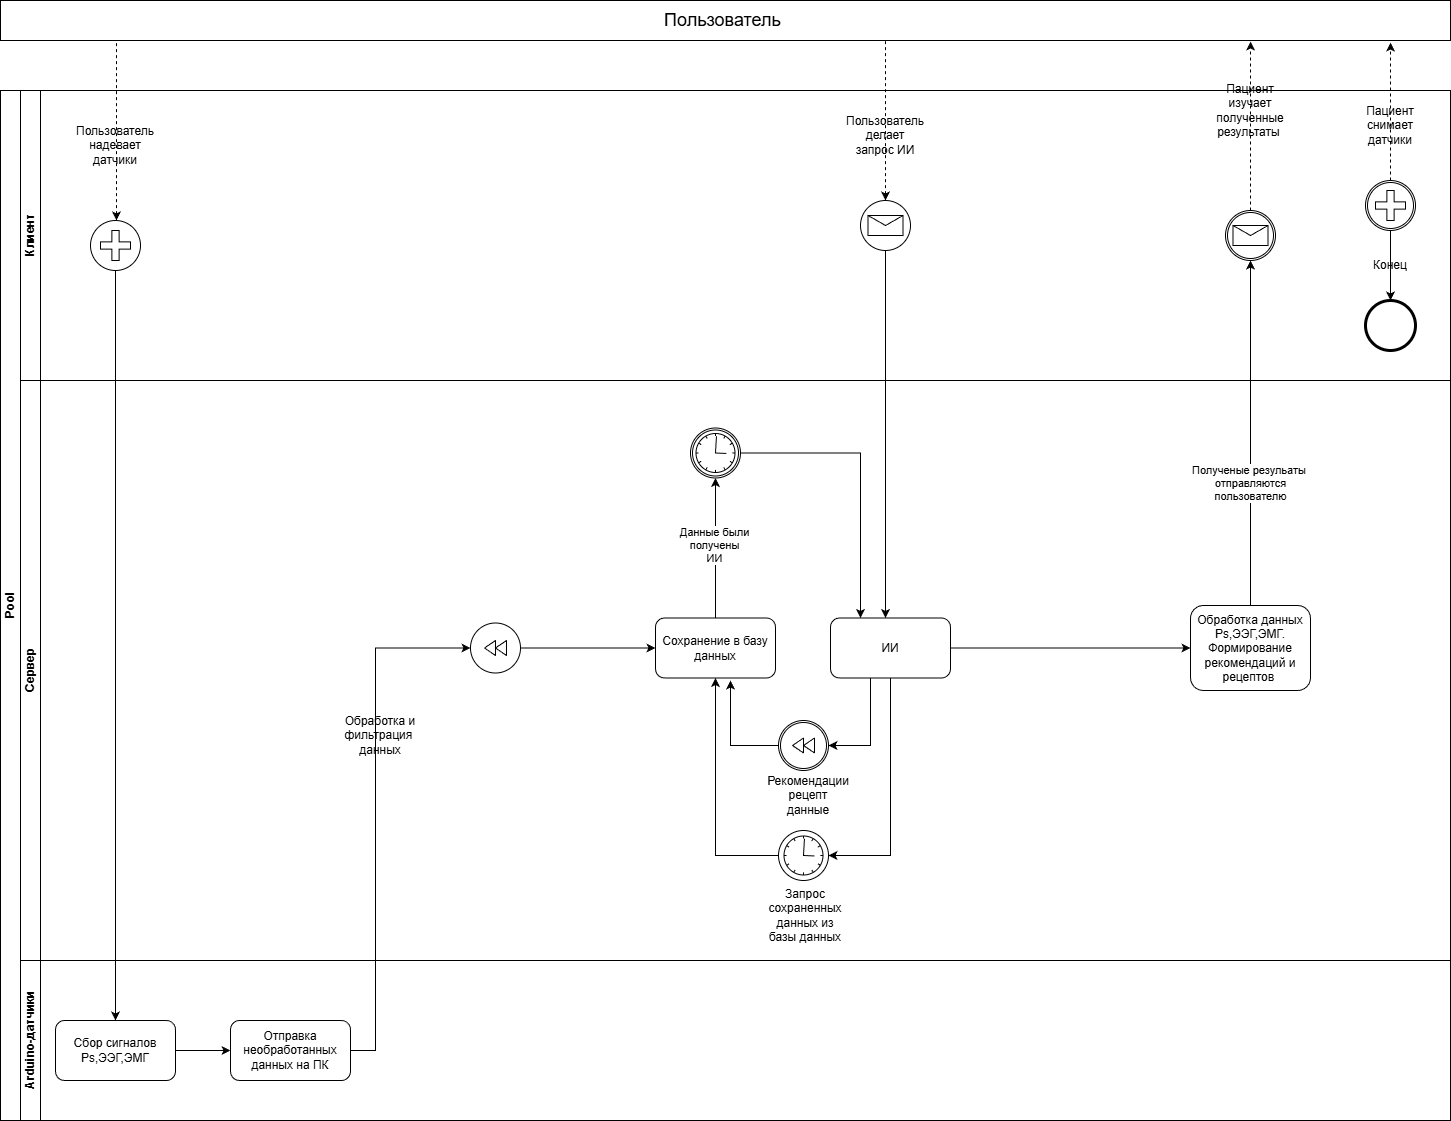
\includegraphics[width=0.9\textwidth,height=0.65\textheight,keepaspectratio]{images/bpmn.png}
    \caption{Алгоритм функционирования устройства}
    \label{fig:bpmn}
\end{sidewaysfigure}

\begin{sidewaysfigure}
    \centering
    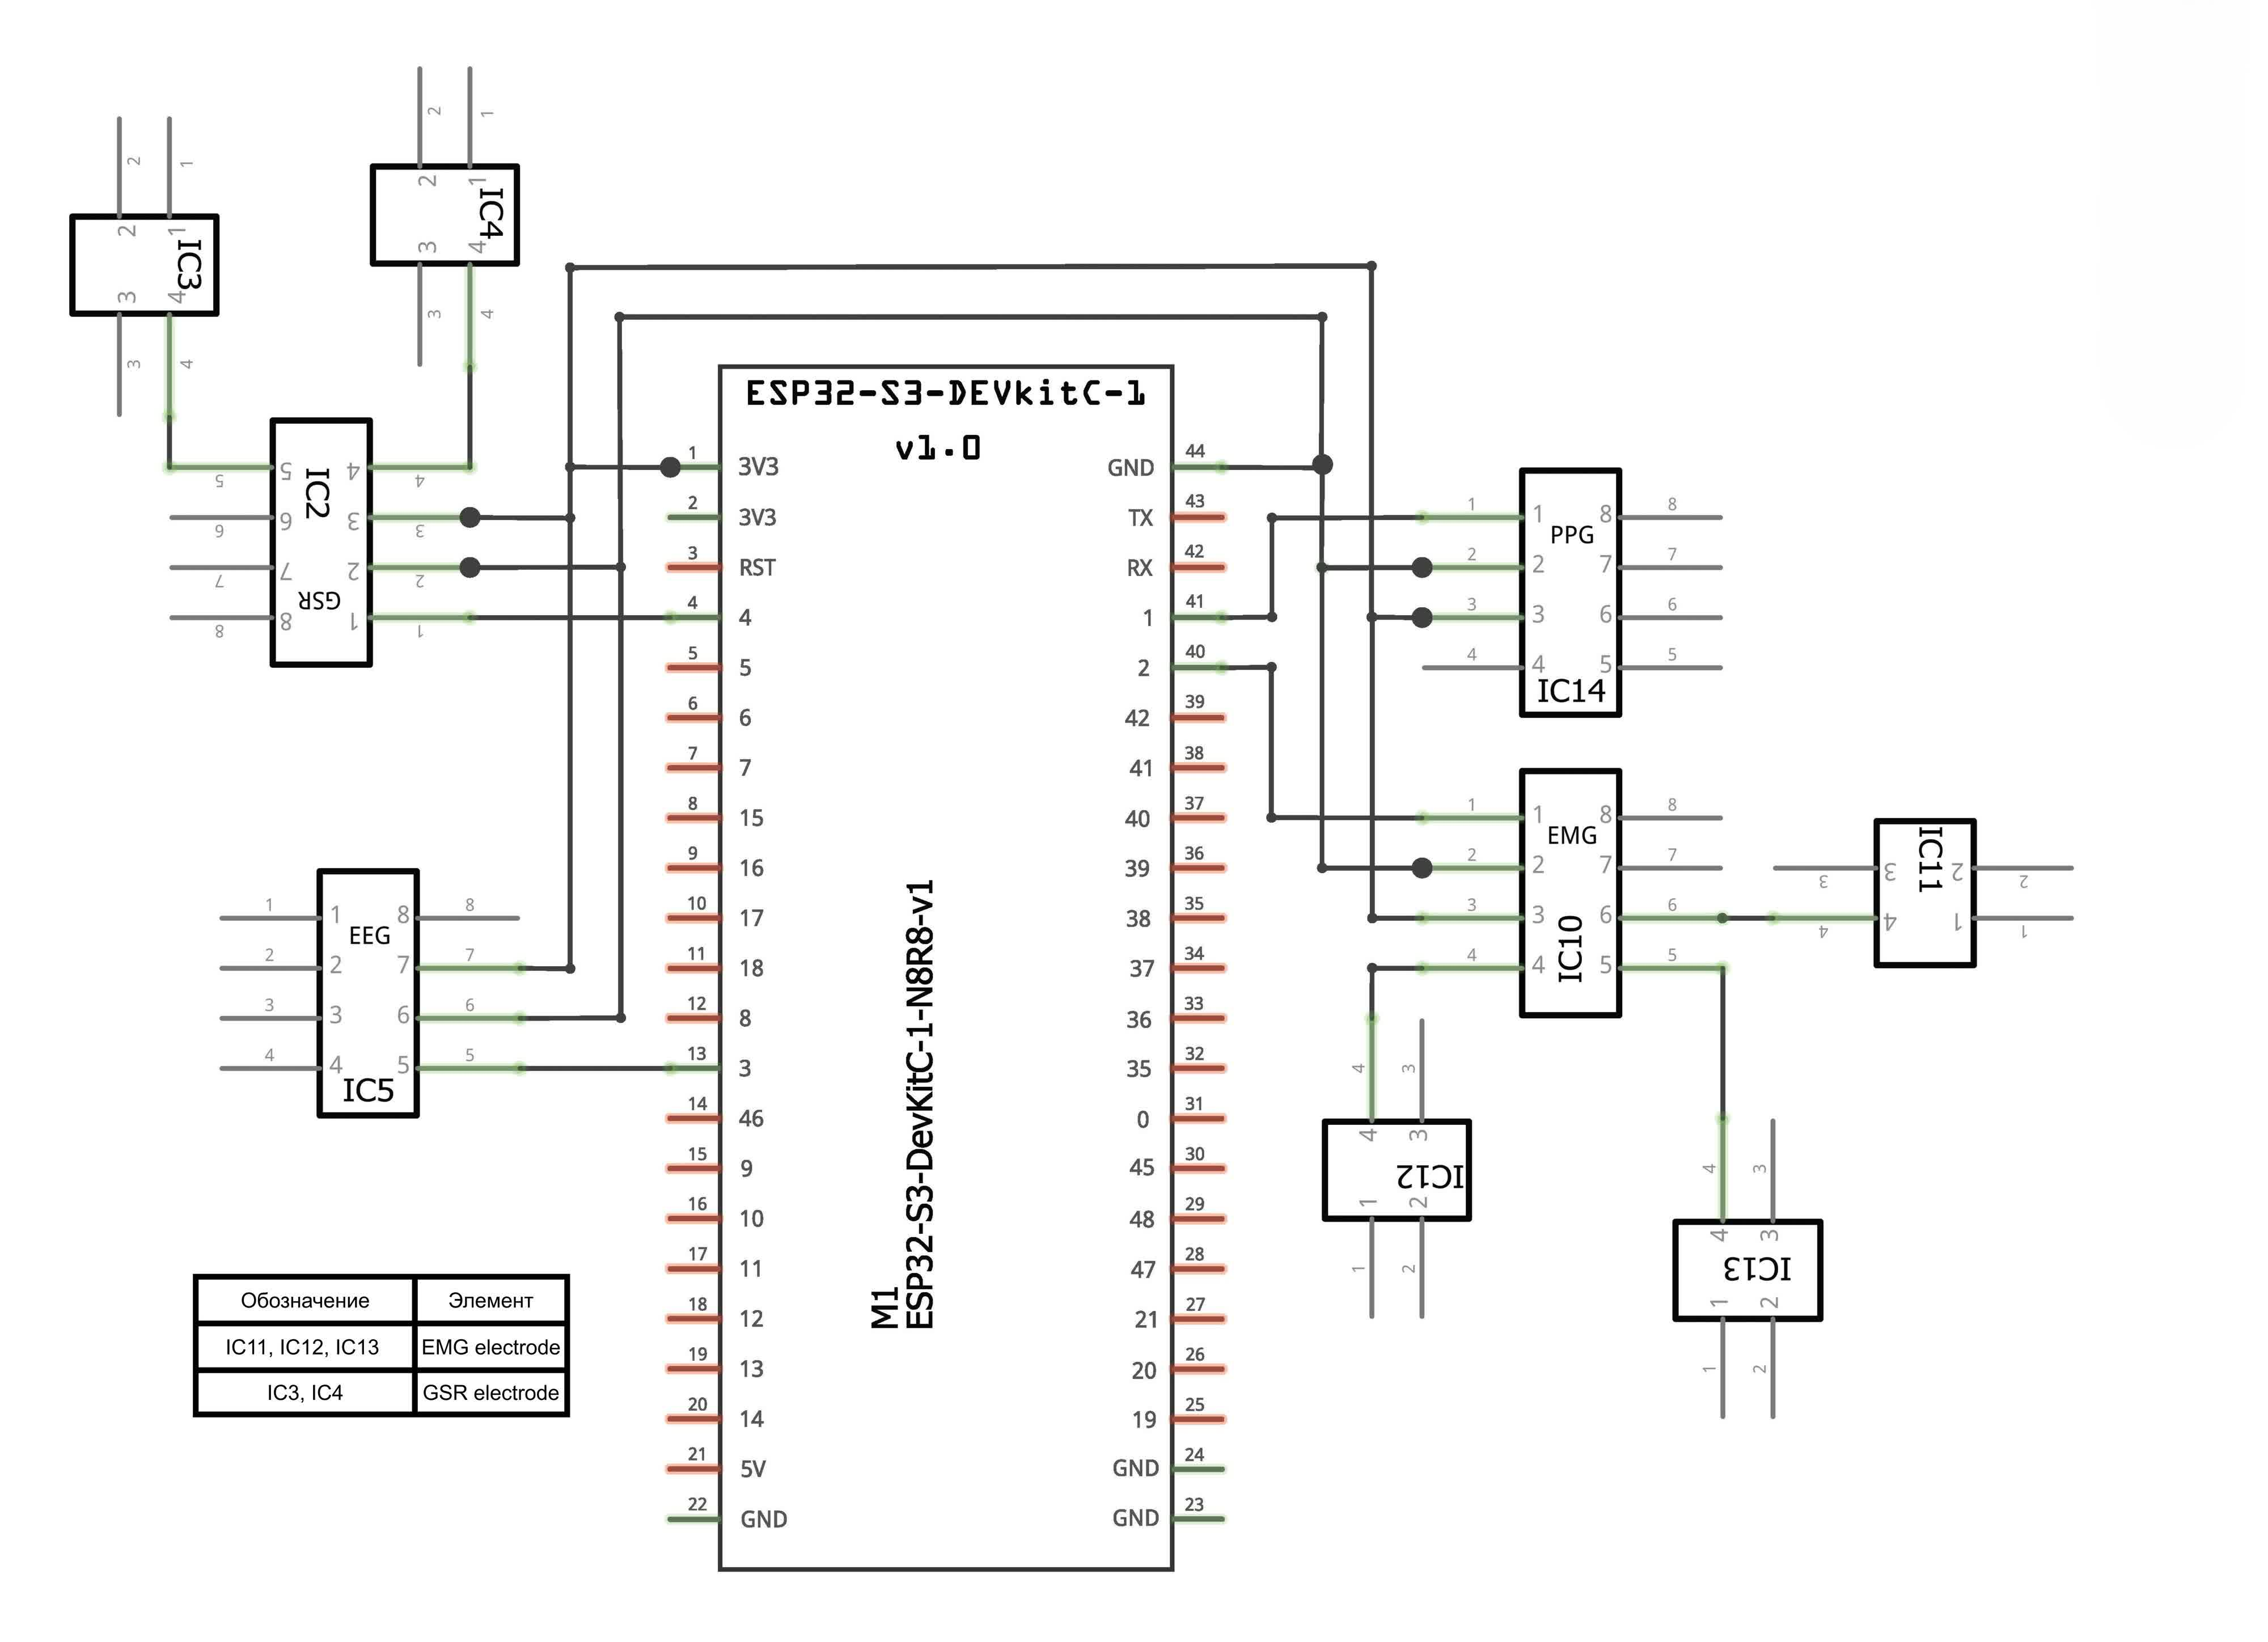
\includegraphics[width=0.9\textwidth,height=0.9\textheight,keepaspectratio]{images/Arduino_схема.jpg}
    \caption{Схема электрическая принципиальная}
    \label{fig:schematic}
\end{sidewaysfigure}

\begin{sidewaysfigure}
    \centering
    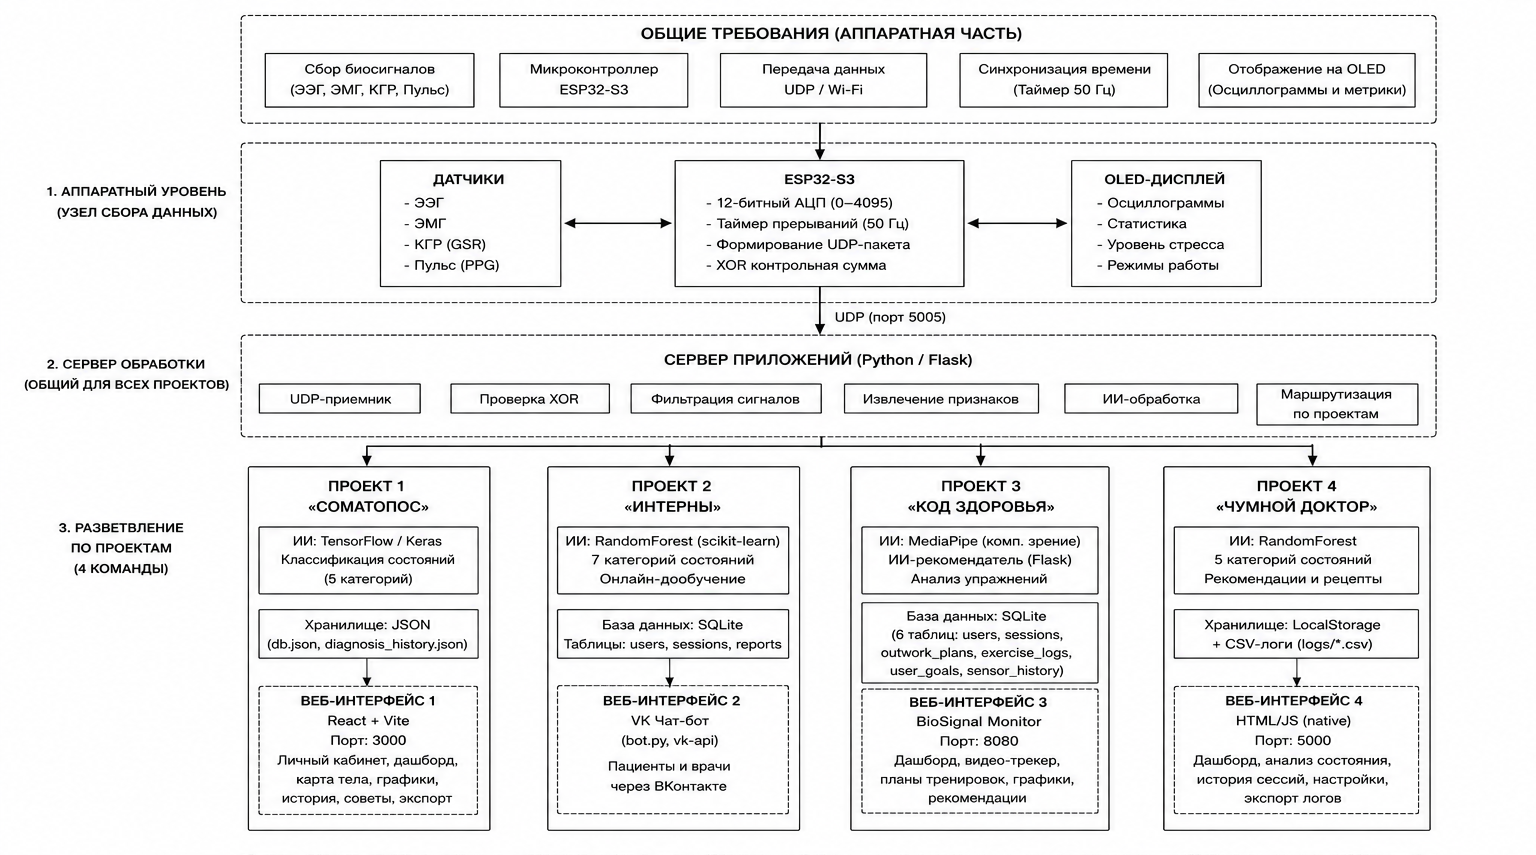
\includegraphics[width=0.95\textwidth,height=0.9\textheight,keepaspectratio]{images/complex_scheme.png}
    \caption{Схема взаимодействия внутри системы}
    \label{fig:complex_scheme}
\end{sidewaysfigure}

\newpage
Цикл работы системы:
\begin{enumerate}
    \item Аппаратные датчики непрерывно регистрируют биосигналы с тела пользователя.
    \item Микроконтроллер ESP32-S3 по аппаратному таймеру опрашивает каналы АЦП, вычисляет контрольную сумму, формирует 11-байтовый буфер и отправляет его по UDP на IP-адрес сервера (порт \texttt{5005}).
    \item Python-сервер принимает UDP-пакеты, проверяет их целостность по XOR-контрольной сумме (отбрасывая битые кадры), выполняет масштабирование и фильтрацию данных.
    \item Модули искусственного интеллекта на стороне сервера обрабатывают очищенные сигналы, классифицируют функциональное состояние пользователя по 5 категориям (<<Напряжение>>, <<Утомление>>, <<Восстановление>>, <<Стресс>>, <<Перегрузка>>) и генерируют рекомендации.
    \item Веб-интерфейс получает обработанные данные по протоколу HTTP (REST API) или HTTP-polling и визуализирует их на графиках в реальном времени.
\end{enumerate}

\subsection{Проект 1: «СОМАТОПОС» (Команда СОМАТОПОС)}
Проект ориентирован на классификацию физиологического состояния по биосигналам пульса, ЭМГ и ЭЭГ с использованием моделей глубокого обучения на базе TensorFlow/Keras.
\begin{itemize}
    \item \textbf{ИИ-компонент}: Нормализация данных с использованием сохраненных параметров скейлера \texttt{scaler.pkl} и классификация через нейросеть (TensorFlow/Keras) по карте меток \texttt{label\_map.json} для выявления рисков сердечно-сосудистой системы, мышечного перенапряжения или аномальной мозговой активности в режиме реального времени. История классификаций сохраняется в файле \texttt{diagnosis\_history.json}.
    \item \textbf{Интерфейс}: Интерактивный дашборд <<Цифровой доктор>>, выполненный в футуристичном дизайне Apple Liquid Glass (порт \texttt{3000}). Отображает графики пульса, ЭМГ и ЭЭГ, текущий вердикт нейросети и процент уверенности модели. В интерфейс интегрирована интерактивная визуальная карта тела (с интерактивной подсветкой зон головы, сердца, мышц кора и конечностей), позволяющая наглядно отображать возможные сбои в организме на основе классификации биосигналов. Данные пользователей (логины, пароли при регистрации) сохраняются локально в файле \texttt{db.json}.
    \item \textbf{Особенности запуска}: Для работы системы требуется запустить три параллельных процесса: \texttt{headless\_diagnostic.py} для приема данных и классификации, \texttt{npm run dev} для веб-интерфейса и \texttt{send\_test.py} для генерации тестового сигнала в отсутствие реальных датчиков.
\end{itemize}

\subsection{Проект 2: «Интерны» (Команда «Интерны»)}
Проект фокусируется на построении надежной клиент-серверной архитектуры с авторизацией пользователей и ведением базы данных измерений.
\begin{itemize}
    \item \textbf{ИИ-компонент}: Использует интерактивную самообучающуюся ИИ-модель на базе классификатора \texttt{RandomForestClassifier} и \texttt{StandardScaler} (библиотека \texttt{scikit-learn}~\cite{sklearn_docs}). Классифицирует состояние на 7 категорий: «Норма», «Напряжение», «Усталость», «Восстановление», «Стресс», «Перегрузка» и «Аритмия». Модель поддерживает динамическое online-дообучение на основе ручных корректировок заключения ИИ, вводимых врачом.
    \item \textbf{База данных}: Хранение истории сессий измерений, учетных записей врачей и пациентов, а также отчетов ИИ в реляционной базе данных под управлением \textbf{SQLite} (таблицы \texttt{users}, \texttt{sessions}, \texttt{reports}).
    \item \textbf{Интерфейс}: Взаимодействие реализовано через чат-бота ВКонтакте (\texttt{bot.py} на базе \texttt{vk-api}). Пациенты могут запустить сессию обследования и просматривать историю своих сессий, а лечащие врачи — просматривать статистику точности ИИ и модерировать заключения (подтверждать или корректировать) непосредственно через кнопочный интерфейс чата, автоматически запуская дообучение модели.
\end{itemize}

\subsection{Проект 3: «Код здоровья» (Команда «Код здоровья»)}
Проект представляет гибридное решение, объединяющее физиологический мониторинг с компьютерным зрением для персональных тренировок и реабилитации.
\begin{itemize}
    \item \textbf{Аппаратная часть}: Дополнительно к стандартной аппаратной части требуется внешняя веб-камера, подключенная к ПК.
    \item \textbf{ИИ-тренер}: Видеоанализ упражнений в реальном времени с использованием библиотеки \texttt{MediaPipe}~\cite{mediapipe_docs} (Pose Landmark Detection). Алгоритм строит скелетную модель пользователя по 33 точкам, рассчитывает тригонометрические углы в суставах (локтевых, коленных) и сравнивает их с эталонными траекториями, мгновенно сообщая об ошибках в технике выполнения и помогая предотвратить травмы при ЛФК и тренировках.
    \item \textbf{ИИ-рекомендатель}: Интеллектуальный помощник Flask-сервера (Python 3.12) генерирует персонализированные планы упражнений на основе заданных целей (общий тонус, похудение, набор массы, выносливость, реабилитация) и уровней сложности (легкий, средний, сложный).
    \item \textbf{Интерфейс}: Панель BioSignal Monitor (порт \texttt{8080}) с карточками показателей, живыми графиками физиологических сигналов и окном видеотрекера с наложением скелетной сетки. Базовые учетные данные по умолчанию: логин/пароль \texttt{123}.
\end{itemize}

\subsection{Проект 4: «Чумной Доктор» (Команда «Чумной Доктор»)}
Проект выделяется развитым консольным CLI-интерфейсом для разработчиков и исследователей, гибкой настройкой порогов ИИ-моделей, а также облачным развертыванием.
\begin{itemize}
    \item \textbf{ИИ-компонент}: Включает Random Forest классификатор для определения 5 функциональных состояний (Напряжение, Утомление, Восстановление, Стресс, Перегрузка). ИИ также формирует рекомендации и рецепты с указанием возможных препаратов.
    \item \textbf{Пошаговый CLI-конвейер}: Процесс разработки разбит на скрипты:
          \begin{enumerate}
              \item \texttt{step1\_train\_v8\_final.py} --- обучение модели классификатора;
              \item \texttt{step2\_test\_v8\_full\_report.py} --- автономное тестирование модели с генерацией подробных отчетов;
              \item \texttt{step3\_realtime\_v8\_2.py} --- мониторинг в реальном времени с выводом в консоль и ведением CSV-логов в папке \texttt{logs\_realtime/} с именами вида \texttt{drhouse\_YYYY-MM-DD\_HH-MM-SS.csv}.
          \end{enumerate}
    \item \textbf{Настройка параметров}: Конфигурационный класс \texttt{Config} позволяет настраивать: частоту анализа \texttt{ANALYZE\_EVERY = 1.0} с, размер истории \texttt{HISTORY\_SIZE = 5}, очистку консоли, пороги пульса для выявления брадикардии (ниже \texttt{50} BPM) и тахикардии (выше \texttt{130} BPM), а также порог уверенности \texttt{CONFIDENCE\_THRESHOLD = 0.55}. Если уверенность модели ниже 55\%, выводится вердикт <<НЕОПРЕДЕЛЁННО>>.
    \item \textbf{Интерфейс}: Веб-интерфейс запускается локально на порту \texttt{5000}. Авторизация: \texttt{admin} / \texttt{123456}. Связь с сервером реализована по протоколу HTTP (REST API), а приём данных с АЦП — через UDP-сокет. Имеется блок «Анализ состояния», история записей с пагинацией, кнопка записи сессий, а также JS-контроллеры для регулировки усиления и калибровки каждого датчика.
\end{itemize}

\subsection{Алгоритмическое обеспечение}
Алгоритмическое обеспечение системы решает задачи фильтрации сырых сигналов, выделения физиологических признаков и классификации состояния пользователя в реальном времени.

\subsubsection{Цифровая фильтрация сигналов}
Сырые биосигналы, поступающие с АЦП микроконтроллера, подвержены влиянию сетевых помех (наводка 50 Гц от электрических сетей) и двигательных артефактов. Для их устранения применяется цифровой режекторный фильтр (Notch filter) 50 Гц. Передаточная функция фильтра в $Z$-области имеет вид:
\begin{equation}
    H(z) = \frac{1 - 2\cos(\omega_0)z^{-1} + z^{-2}}{1 - 2r\cos(\omega_0)z^{-1} + r^2 z^{-2}}
\end{equation}
где $\omega_0 = \frac{2\pi f_0}{f_s}$, $f_0 = 50$~Гц (частота режекции), $f_s$~--- частота дискретизации сигнала ($f_s > 2f_0$ по теореме Найквиста), а $r \in [0.95, 0.99]$ — коэффициент, задающий ширину полосы подавления.

Разностное уравнение для реализации фильтра во временной области:
\begin{equation}
    y[n] = x[n] - 2\cos(\omega_0)x[n-1] + x[n-2] + 2r\cos(\omega_0)y[n-1] - r^2 y[n-2]
\end{equation}
где $x[n]$ — входной отсчет сигнала, $y[n]$ — отфильтрованный отсчет.

\subsubsection{Детектирование пиков пульсовой волны и расчет ЧСС}
Для расчета частоты сердечных сокращений (BPM) в реальном времени используется пороговый алгоритм детектирования пиков пульсовой волны:
\begin{enumerate}
    \item Сигнал опрашивается с частотой 50 Гц.
    \item Фиксируется переход сигнала через верхний порог $T_{peak} = 2800$ (для 12-битного АЦП):
          \begin{equation}
              S[n] > T_{peak} \quad \text{и} \quad S[n-1] \le T_{peak}
          \end{equation}
    \item Измеряется временной интервал $\Delta t = t_n - t_{n-1}$ (в миллисекундах) между двумя последовательными пиками (NN-интервал).
    \item Если интервал лежит в физиологических границах $400~\text{мс} < \Delta t < 1500~\text{мс}$ (что соответствует ЧСС от 40 до 150 уд/мин), производится расчет мгновенной ЧСС:
          \begin{equation}
              BPM = \frac{60000}{\Delta t}
          \end{equation}
\end{enumerate}

\subsubsection{Статистический анализ вариабельности ритма сердца (ВРС)}
Для оценки активности вегетативной нервной системы (баланса симпатического и парасимпатического отделов) рассчитываются временные показатели ВРС:
\begin{itemize}
    \item Среднеквадратичное отклонение разностей последовательных NN-интервалов (RMSSD), отражающее парасимпатическую активность:
          \begin{equation}
              RMSSD = \sqrt{\frac{1}{N-1}\sum_{i=1}^{N-1} (\Delta t_{i+1} - \Delta t_i)^2}
          \end{equation}
    \item Стандартное отклонение NN-интервалов (SDNN), характеризующее общую вариабельность:
          \begin{equation}
              SDNN = \sqrt{\frac{1}{N}\sum_{i=1}^N (\Delta t_i - \overline{\Delta t})^2}
          \end{equation}
\end{itemize}

\subsubsection{Масштабирование показателей КГР (GSR) в уровень стресса}
Проводимость кожи (обратная величина сопротивления) напрямую коррелирует с уровнем стресса и активностью потовых желез. Значение АЦП масштабируется в процентный показатель по формуле:
\begin{equation}
    Stress_{\%} = \frac{GSR_{raw} - GSR_{min}}{GSR_{max} - GSR_{min}} \times 100
\end{equation}
где $GSR_{min} = 500$, $GSR_{max} = 3800$ — минимальные и максимальные калибровочные границы АЦП. Итоговое значение ограничивается диапазоном $[0, 100]\%$.

\subsubsection{Расчет мышечного напряжения по ЭМГ}
Амплитуда электромиограммы отражает силу сокращения мышц. Для оценки мышечной нагрузки вычисляется размах сигнала в скользящем окне размером $W = 50$ отсчетов ($1$ секунда):
\begin{equation}
    A_{EMG} = \max_{k \in [0, W-1]} (EMG[n-k]) - \min_{k \in [0, W-1]} (EMG[n-k])
\end{equation}
Если $A_{EMG} > 100$ единиц АЦП, мышечное напряжение рассчитывается по формуле:
\begin{equation}
    MuscleLoad_{\%} = \frac{A_{EMG} - 100}{24}
\end{equation}
Результат приводится к диапазону $[0, 100]\%$.

\subsubsection{Анализ спектральных ритмов ЭЭГ}
Нормализованное значение мозговой активности $EEG_{norm}$ приводится к диапазону $[0, 100]\%$ на основе максимального значения АЦП ($4095$):
\begin{equation}
    EEG_{norm} = \frac{EEG_{raw}}{4095} \times 100
\end{equation}
Соотношение альфа- и бета-ритмов оценивается приближенно по формулам:
\begin{equation}
    AlphaRatio_{\%} = 30 + 0.5 \times (100 - EEG_{norm})
\end{equation}
\begin{equation}
    BetaRatio_{\%} = 0.8 \times EEG_{raw} / 40.95
\end{equation}

\subsection{Информационное обеспечение}

Информационное обеспечение интегрированной программно-аппаратной системы построено с учетом различных подходов команд к организации хранения данных. Архитектура объединяет как реляционные СУБД для надежного транзакционного хранения, так и документо-ориентированные форматы (JSON) и файловые структуры (CSV) для логов.

\subsubsection{Общая абстрактная ERD-схема системы}
Для интеграции всех модулей была спроектирована общая концептуальная схема данных (рисунок~\ref{fig:erd_abstract}), отражающая логическую сущность процесса мониторинга. Она включает в себя следующие основные сущности:
\begin{itemize}
    \item \textbf{\texttt{users}:} содержит данные зарегистрированных в системе пользователей (пациентов, врачей, администраторов) и включает: уникальный идентификатор (`id`), имя пользователя (`username`), зашифрованный пароль (`password`), роль в системе (`role`) и метку времени создания учетной записи (`created\_at`);
    \item \textbf{\texttt{sessions}:} хранит информацию о сеансах физиологического мониторинга и включает: уникальный идентификатор сессии (`id`), внешний ключ пользователя (`user\_id`), время запуска сессии (`created\_at`), статус завершения (`status`), а также усредненные показатели датчиков за сессию --- частоту сердечных сокращений (`bpm`), мышечное напряжение (`muscle`), активность мозга (`brain`) и общий уровень стресса (`stress`);
    \item \textbf{\texttt{reports}:} фиксирует ИИ-заключения и врачебные отчеты по результатам сессий и включает: уникальный идентификатор отчета (`id`), внешний ключ сессии (`session\_id`), внешний ключ лечащего врача (`doctor\_id`), автоматический вердикт нейросети (`ai\_conclusion`), рекомендации и предписания врача (`doctor\_conclusion`), текущий статус проверки отчета (`status`) и время создания (`created\_at`).
\end{itemize}

\newpage

\begin{figure}[H]
    \centering
    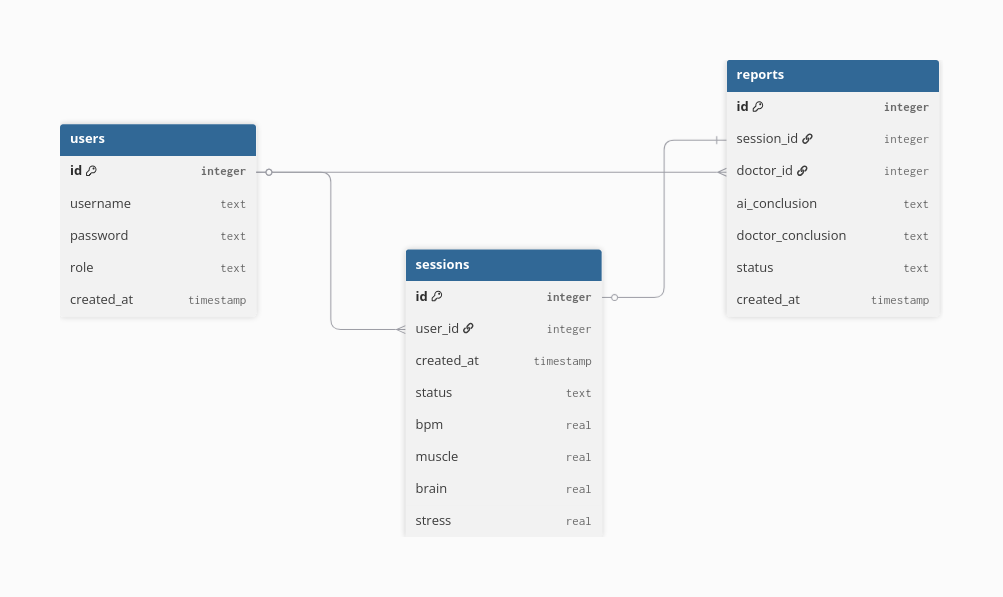
\includegraphics[width=0.95\textwidth,height=0.95\textheight,keepaspectratio]{images/erd_abstract.png}
    \caption{Общая абстрактная ERD-схема системы}
    \label{fig:erd_abstract}
\end{figure}

\newpage

\subsubsection{Схема данных проекта «СОМАТОПОС» (Команда 1)}
Проект СОМАТОПОС ориентирован на файловое хранение данных в формате JSON. Схема связей логических сущностей представлена на рисунке~\ref{fig:erd_somatopos}. Хранилище включает в себя следующие основные таблицы и структуры:
\begin{itemize}
    \item \textbf{\texttt{users}:} содержит учетные данные пользователей для авторизации в системе и включает: уникальное имя пользователя (`name`), выступающее в качестве первичного ключа, и пароль (`password`);
    \item \textbf{\texttt{history}:} хранит исторические логи сеансов мониторинга и включает: имя пользователя (`user`), дату проведения измерения (`date`), среднюю ЧСС (`hr`), показатели активности мышц (`muscle`) и мозга (`brain`), а также общее состояние пользователя (`state`);
    \item \textbf{\texttt{diagnosis\_history}:} содержит логи классификации состояний нейросетью с высокой частотой дискретизации и включает: временную метку (`timestamp`), выступающую первичным ключом, строковое представление даты и времени (`datetime`), текущую ЧСС (`bpm`), расчетные показатели ЭМГ (`muscle`) и ЭЭГ (`eeg`), код классифицированного диагноза (`diagnosis\_code`), краткое (`diagnosis\_short`) и развернутое (`diagnosis\_full`) текстовые заключения ИИ, процент уверенности модели (`confidence`), а также сырые оцифрованные сигналы АЦП датчиков пульса (`raw\_pulse`), ЭМГ (`raw\_emg`) и ЭЭГ (`raw\_eeg`).
\end{itemize}

\begin{figure}[H]
    \centering
    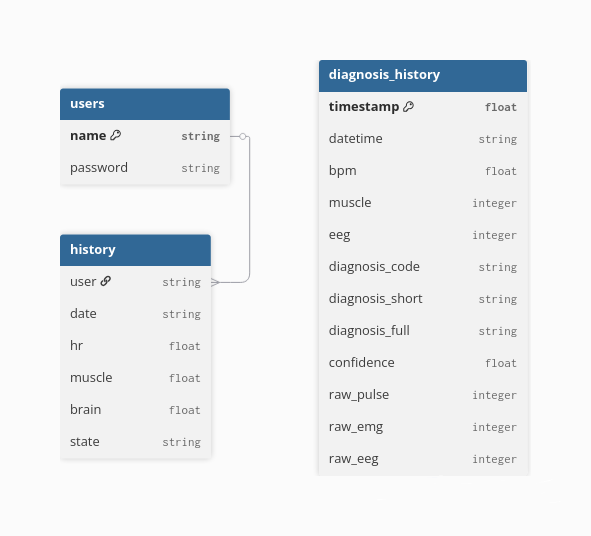
\includegraphics[width=0.75\textwidth,height=0.6\textheight,keepaspectratio]{images/erd_somatopos.png}
    \caption{ERD-схема базы данных проекта «СОМАТОПОС»}
    \label{fig:erd_somatopos}
\end{figure}

\subsubsection{Схема данных проекта «Интерны» (Команда 2)}
Реализована реляционная база данных под управлением СУБД SQLite. Архитектура базы данных представлена на рисунке~\ref{fig:erd_interns} и включает три основные сущности (сценарий инициализации схемы базы данных SQLite приведен в Приложении А, подраздел А.5):
\begin{itemize}
    \item \textbf{\texttt{users}:} хранит информацию о пользователях системы и включает: уникальный идентификатор (`id`), идентификатор пользователя в социальной сети ВКонтакте (`vk\_id`) для работы чат-бота, имя пользователя (`name`), роль пользователя (`role`) и дату регистрации (`created\_at`);
    \item \textbf{\texttt{sessions}:} фиксирует запущенные сессии медицинского обследования пациентов и включает: уникальный идентификатор сессии (`id`), внешний ключ пациента (`user\_id`), текущий статус обследования (`status`), сырые текстовые данные измерений в формате JSON (`raw\_data`) и время старта сессии (`created\_at`);
    \item \textbf{\texttt{reports}:} содержит заключение и отчеты по сессиям и включает: уникальный идентификатор отчета (`id`), внешний ключ обследования (`session\_id`), автоматические рекомендации искусственного интеллекта (`ai\_conclusion`), экспертное заключение лечащего врача (`doctor\_conclusion`), внешний ключ врача (`doctor\_id`), статус верификации отчета (`status`) и время формирования (`created\_at`).
\end{itemize}

\begin{figure}[H]
    \centering
    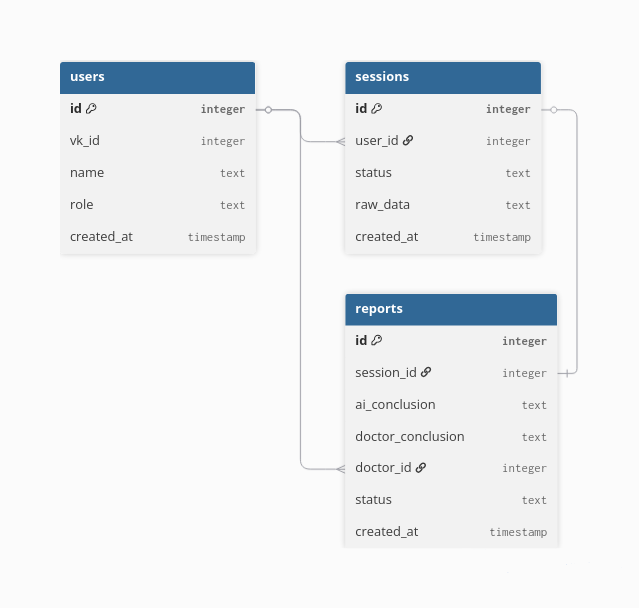
\includegraphics[width=0.75\textwidth,height=0.7\textheight,keepaspectratio]{images/erd_interns.png}
    \caption{ERD-схема базы данных проекта «Интерны»}
    \label{fig:erd_interns}
\end{figure}

\subsubsection{Схема данных проекта «Код здоровья» (Команда 3)}
База данных проекта, реализованная в MedApp на базе SQLite, имеет расширенную реляционную структуру (рисунок~\ref{fig:erd_health}). Она включает следующие сущности для ИИ-тренировок и мониторинга:
\begin{itemize}
    \item \textbf{\texttt{users}:} содержит профильные и учетные данные участников системы и включает: уникальный идентификатор пользователя (`id`), логин для авторизации (`username`), адрес электронной почты (`email`), ФИО (`full\_name`), дату рождения (`birth\_date`), роль в системе (`role`), хеш пароля (`password`) и дату регистрации (`created\_at`);
    \item \textbf{\texttt{sessions}:} фиксирует метаданные тренировочных и реабилитационных сессий и включает: уникальный идентификатор сессии (`id`), внешний ключ пользователя (`user\_id`), название тренировки (`name`), время начала (`start\_time`) и завершения (`end\_time`), количество записанных точек данных (`data\_points`), время сохранения сессии (`created\_at`) и дополнительную мета-информацию в формате JSON (`meta\_json`);
    \item \textbf{\texttt{workout\_plans}:} содержит тренировочные программы, сгенерированные ИИ-помощником, и включает: уникальный идентификатор плана (`id`), внешний ключ пользователя (`user\_id`), описание упражнений в формате JSON (`plan\_json`), уровень сложности (`difficulty`), цель программы (`goal`) и время создания (`created\_at`);
    \item \textbf{\texttt{exercise\_logs}:} записывает детальную историю выполнения отдельных упражнений в рамках планов и включает: уникальный идентификатор записи (`id`), внешний ключ пользователя (`user\_id`), внешний ключ плана тренировок (`plan\_id`), строковый идентификатор упражнения (`exercise\_id`), название упражнения (`exercise\_name`), количество выполненных повторений (`reps`), субъективную сложность (`difficulty`), длительность выполнения в секундах (`duration\_sec`) и время завершения (`completed\_at`);
    \item \textbf{\texttt{user\_goals}:} содержит спортивные и реабилитационные цели пользователей и включает: уникальный идентификатор цели (`id`), внешний ключ пользователя (`user\_id`), текстовое описание цели (`goal\_text`), целевое число повторений (`target\_reps`), целевое упражнение (`target\_exercise`), статус достижения цели (`achieved`) и время создания (`created\_at`);
    \item \textbf{\texttt{sensor\_history}:} хранит временные ряды показаний сенсоров биосигналов и включает: уникальный идентификатор записи (`id`), внешний ключ логина пользователя (`username`), текущую ЧСС (`bpm`), уровень стресса (`stress`), активность мышц (`muscle`), спектральные показатели альфа- (`alpha`) и бета-ритмов ЭЭГ (`beta`), текущее состояние (`state`) и время записи (`recorded\_at`).
\end{itemize}

\begin{figure}[H]
    \centering
    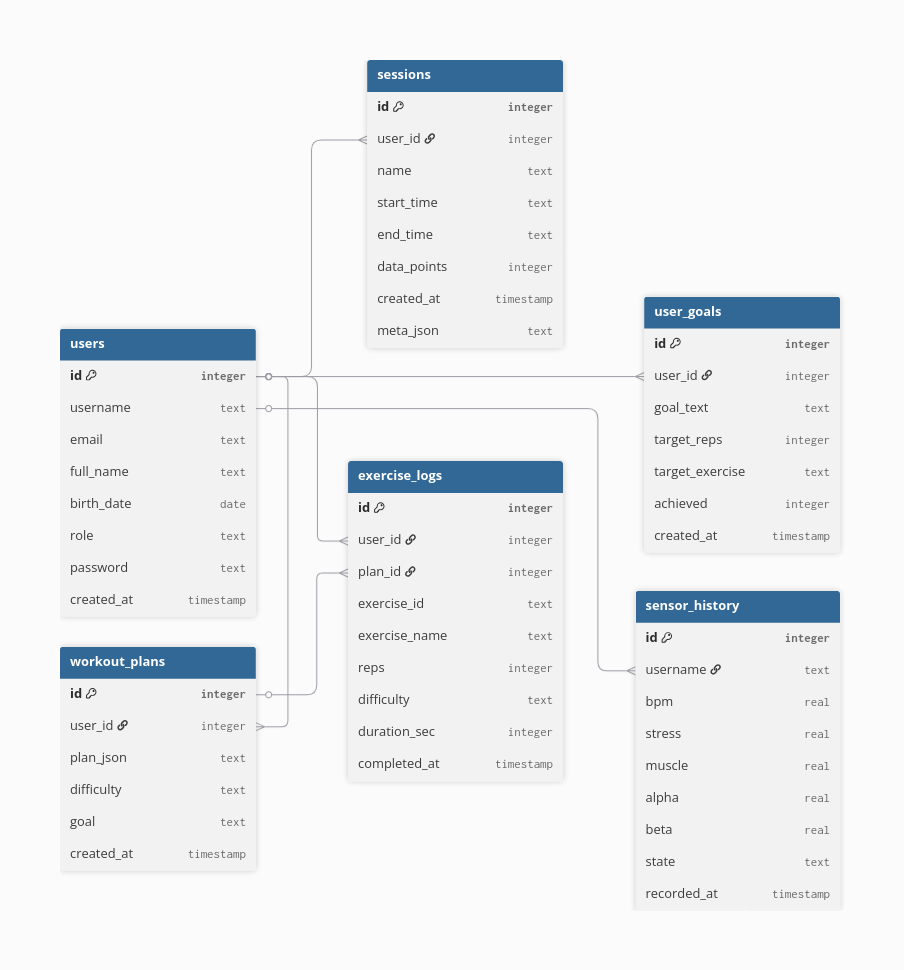
\includegraphics[width=0.95\textwidth,height=0.7\textheight,keepaspectratio]{images/erd_health.png}
    \caption{ERD-схема базы данных проекта «Код здоровья»}
    \label{fig:erd_health}
\end{figure}

\subsubsection{Схема данных проекта «Чумной Доктор» (Команда 4)}
Проект совмещает локальную клиентскую базу данных LocalStorage для хранения пользовательских сессий и ведение CSV-логов на стороне Python-сервера для детального анализа сигналов. Архитектура логического хранения представлена на рисунке~\ref{fig:erd_plague}. База данных и лог-файлы включают в себя следующие сущности и поля:
\begin{itemize}
    \item \textbf{\texttt{users} (LocalStorage):} хранит информацию об учетных записях пользователей для авторизации в локальной панели управления и включает: уникальный идентификатор пользователя (`id`), имя пользователя (`username`), пароль (`pass`) и роль в системе (`role`);
    \item \textbf{\texttt{rows} (LocalStorage):} содержит агрегированные результаты сеансов физиологического мониторинга и включает: уникальный идентификатор записи (`id`), внешний ключ пользователя (`uid`), дату проведения измерения (`date`), среднюю частоту пульса (`bpm`), средний уровень стресса (`stress`), среднее мышечное напряжение (`muscle`), среднюю долю альфа-ритма ЭЭГ (`alpha`), среднюю долю бета-ритма ЭЭГ (`beta`), текстовое определение физиологического состояния (`state`), выписанные врачебные рекомендации (`recipe`) и имя лечащего врача (`doctor`);
    \item \textbf{CSV-логи (Python-сервер):} представляют собой файлы непрерывной записи показаний датчиков с высокой частотой дискретизации для последующего оффлайн-анализа. Каждая строка лог-файла содержит следующие поля: временную метку получения данных (`Время`), порядковый номер пакета для контроля потерь (`Пакет`), скользящее среднее частоты сердечных сокращений (`Пульс\_mean`), среднюю амплитуду ЭМГ (`ЭМГ\_mean`), среднее значение проводимости кожи КГР (`КГР\_mean`), нормализованный показатель ЭЭГ (`ЭЭГ\_mean`), классифицированное нейросетью состояние (`Состояние`), вероятность правильности распознавания (`Уверенность\_\%`) и код критического состояния в случае выхода параметров за нормы (`Критическое`).
\end{itemize}

\begin{figure}[H]
    \centering
    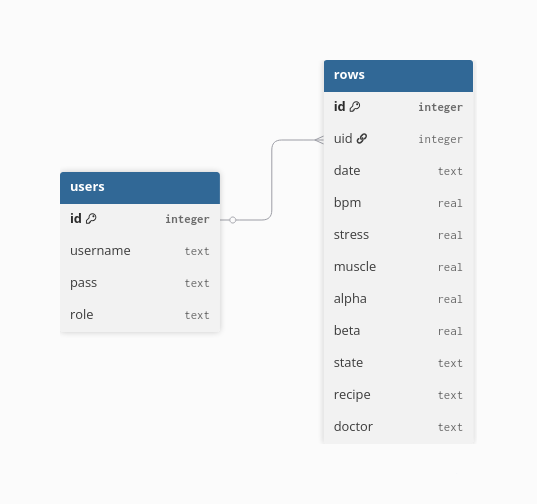
\includegraphics[width=0.75\textwidth,height=0.55\textheight,keepaspectratio]{images/erd_plague.png}
    \caption{ERD-схема базы данных проекта «Чумной Доктор»}
    \label{fig:erd_plague}
\end{figure}

\section{Выбор и обоснование инструментов реализации}
Для реализации системы были выбраны современные инструменты, обеспечивающие высокую производительность и низкую задержку.

\subsection{Общие критерии выбора}
Сравнение архитектурных и технологических решений команд представлено в таблице~\ref{tab:health_comparison}.

\begin{table}[h!tp]
    \centering
    \caption{Технологические решения команд для интегрированной системы}
    \label{tab:health_comparison}
    \small\begin{tabular}{|P{2.8cm}|P{2.7cm}|P{2.7cm}|P{2.7cm}|P{2.7cm}|}
        \hline
        \textbf{Критерий}         & \textbf{Команда 1} & \textbf{Команда 2}            & \textbf{Команда 3}      & \textbf{Команда 4}            \\
        \hline
        \textbf{Аппаратная часть} & ESP32-S3 (UDP)     & ESP32-S3 (UDP)                & ESP32-S3 (UDP) + Камера & ESP32-S3 (UDP)                \\
        \hline
        \textbf{Библиотеки ИИ}    & TensorFlow / Keras & Scikit-learn (Random\-Forest) & MediaPipe / OpenCV      & Scikit-learn (Random\-Forest) \\
        \hline
        \textbf{Веб-интерфейс}    & React + Vite       & Чат-бот VK                    & HTML + CSS              & HTML/JS (native)              \\
        \hline
        \textbf{Backend}          & Node.js / Express  & Flask / UDP                   & Flask                   & Flask / UDP                   \\
        \hline
        \textbf{База данных}      & db.json            & SQLite                        & SQLite                  & LocalStorage + CSV            \\
        \hline
    \end{tabular}
\end{table}

\subsection{Обоснование выбора микроконтроллера ESP32-S3}
В качестве центрального вычислительного элемента аппаратной части системы выбран микроконтроллер \textbf{ESP32-S3} от компании Espressif Systems. Выбор обусловлен следующими ключевыми техническими характеристиками:
\begin{itemize}
    \item \textbf{Высокая производительность:} Микроконтроллер оснащен двухъядерным 32-разрядным процессором Xtensa LX7 с тактовой частотой до 240 МГц. Это обеспечивает достаточную вычислительную мощность для одновременного опроса АЦП на высокой частоте, математического расчета базовых медицинских метрик (ВРС, размаха ЭМГ) и вывода графиков на OLED-дисплей.
    \item \textbf{Аппаратная поддержка векторных инструкций:} ESP32-S3 поддерживает специализированные векторные инструкции (Vector Instructions Extension), ускоряющие выполнение операций цифровой обработки сигналов (DSP) и нейросетевого инференса (библиотека ESP-NN).
    \item \textbf{Интегрированный беспроводной приемопередатчик:} Наличие встроенного модуля Wi-Fi 802.11b/g/n позволяет реализовать беспроводную передачу биометрических данных без использования дополнительных модулей, что уменьшает габариты и энергопотребление устройства.
    \item \textbf{Многоканальный 12-разрядный АЦП:} Наличие двух АЦП (ADC1 и ADC2) с разрешением до 12 бит (4096 уровней квантования) позволяет считывать аналоговые значения с датчиков с высокой точностью.
\end{itemize}

\subsection{Обоснование выбора протокола передачи данных UDP}
Для передачи телеметрических данных с датчиков на сервер был выбран транспортный протокол \textbf{UDP} (User Datagram Protocol) вместо традиционного TCP по следующим причинам:
\begin{itemize}
    \item \textbf{Минимальная задержка (Low Latency):} Протокол UDP не требует установления соединения (handshake) и не выполняет повторный запрос потерянных пакетов. Это критически важно при потоковой передаче сигналов в реальном времени, когда задержка передачи важнее гарантированной доставки каждого отсчета. Потеря отдельных пакетов не влияет на общую картину сигнала, в то время как задержки повторной отправки TCP могут вызвать лавинообразное накопление буфера на передатчике.
    \item \textbf{Минимальные накладные расходы:} Заголовок UDP-пакета составляет всего 8 байт (против 20 байт у TCP), что снижает трафик и экономит ресурс передатчика ESP32-S3.
    \item \textbf{Механизм широковещательной рассылки (Broadcast):} Использование широковещательного адреса \texttt{255.255.255.255} позволяет микроконтроллеру отправлять данные в локальную сеть без жесткой привязки к конкретному IP-адресу сервера, что упрощает запуск системы в динамических сетях (DHCP).
\end{itemize}
Для компенсации ненадежности доставки UDP в структуру пакета введена контрольная сумма (XOR), позволяющая отбрасывать искаженные пакеты на сервере.

\subsection{Языки программирования}
Основным языком разработки серверной части выбран \textbf{Python} (версии 3.8–3.12). Преимущества: наличие зрелых библиотек обработки сигналов (\texttt{scipy}, \texttt{numpy}) и машинного обучения (\texttt{scikit-learn}, \texttt{tensorflow}). Для прошивки микроконтроллеров использовался язык \textbf{C++} (в среде Arduino IDE / PlatformIO) для обеспечения работы АЦП в реальном времени.

\subsection{Графические и веб-фреймворки}
Для дашбордов использовался стек \textbf{React + Vite} (Команда 1) для создания отзывчивого пользовательского интерфейса с обновлением графиков без перезагрузки страниц. Микросервисы API реализованы на фреймворках \textbf{Flask} и \textbf{Express}.

\subsection{Базы данных}
Для хранения учетных записей и истории сессий используется легкая реляционная СУБД \textbf{SQLite}, не требующая развертывания отдельного сервера, что упрощает запуск комплекса на ПК пользователя. Команда 4 дублирует запись сессий в CSV-файлы в папке \texttt{logs/} для удобства экспорта в стороннее исследовательское программное обеспечение (например, MATLAB).

\subsection{Искусственный интеллект}
\begin{itemize}
    \item \textbf{Анализ биосигналов}: Модели классифицируют состояние на основе спектральных признаков ЭМГ и временных параметров вариабельности пульса (RMSSD, pNN50).
    \item \textbf{Компьютерное зрение}: Библиотека \texttt{MediaPipe} строит скелетную модель пользователя по 33 точкам. Алгоритм рассчитывает тригонометрические углы между суставами для оценки амплитуды движений.
\end{itemize}

\section{Реализация системы}
Система реализована в виде распределенного комплекса скриптов. Диаграмма развертывания интегрированной системы представлена на рисунке~\ref{fig:deployment}.

\begin{sidewaysfigure}
    \centering
    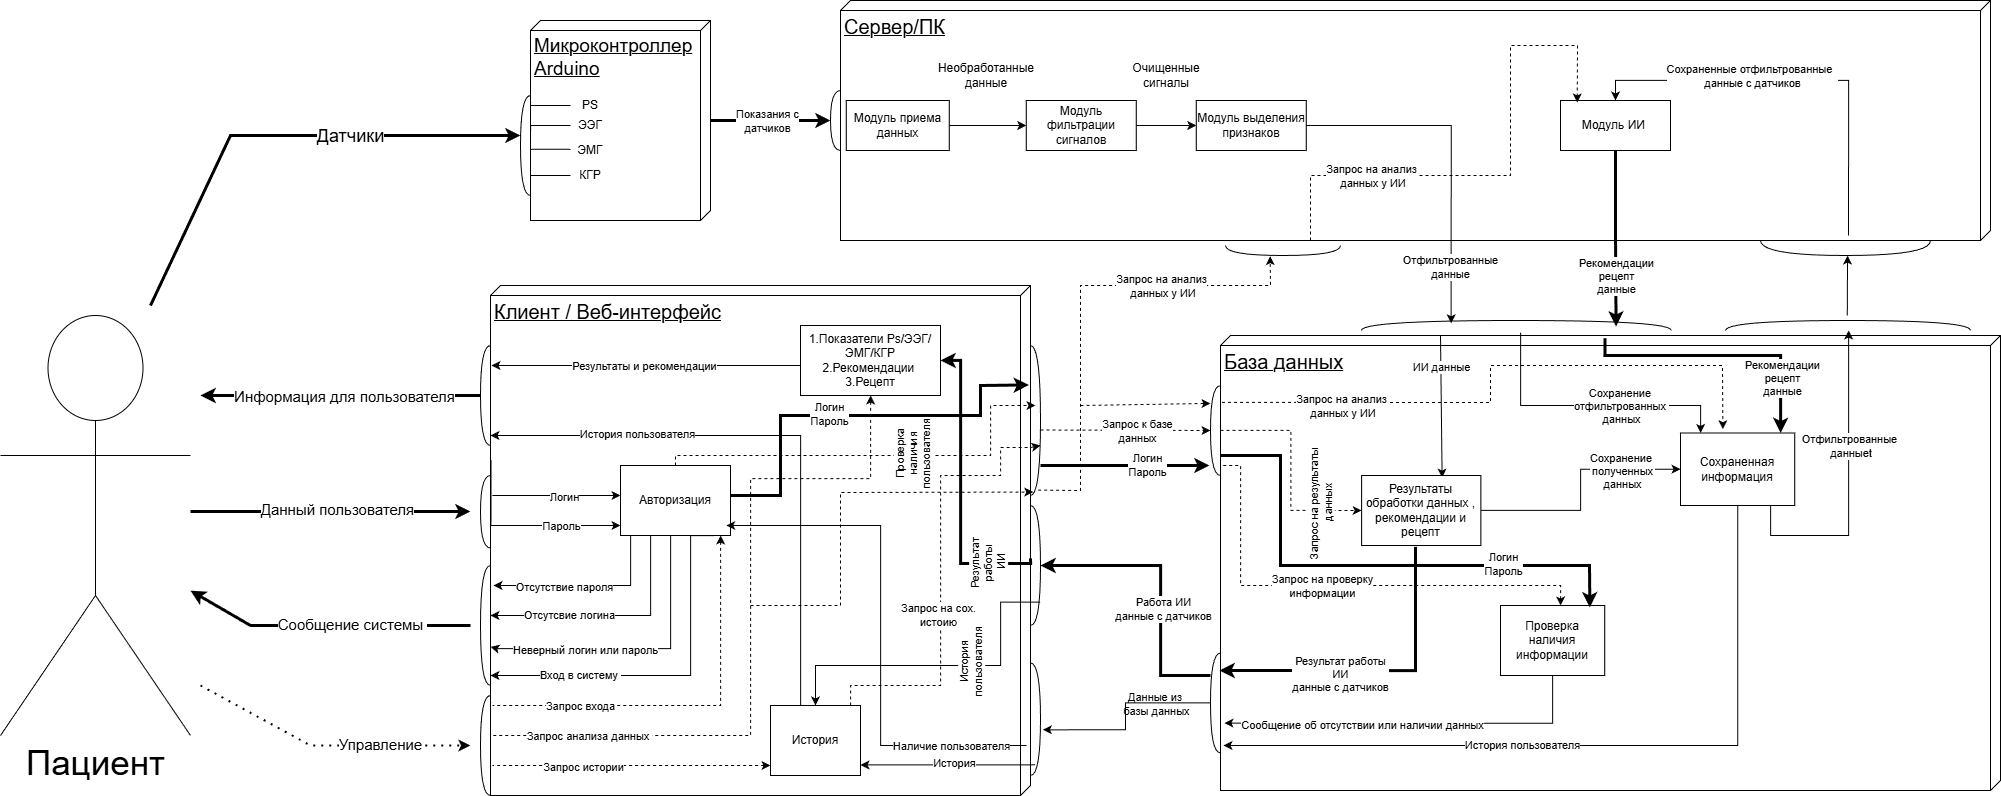
\includegraphics[width=0.9\textwidth,height=0.9\textheight,keepaspectratio]{images/диаграмма_разв.png}
    \caption{Диаграмма развертывания}
    \label{fig:deployment}
\end{sidewaysfigure}

\subsection{Общие модули}
Ключевым общим компонентом является модуль приема UDP-пакетов от микроконтроллера по беспроводной сети Wi-Fi. Структура принимаемого 11-байтового пакета является единой для всего программно-аппаратного комплекса и подробно описана в подразделе~\ref{subsec:common_process} («Общая схема процесса» с разбиением по байтам от стартового \texttt{0xAA} до стопового \texttt{0x55} и вычислением XOR CRC). На стороне сервера приемник считывает входящий UDP-поток на порту \texttt{5005}, производит валидацию контрольной суммы и передает отфильтрованный кадр в обработчики соответствующих проектов. Фрагмент кода для приема и парсинга UDP-пакетов приведен в Приложении А (подраздел А.2).

\subsection{Особенности программного обеспечения микроконтроллера}
Прошивка микроконтроллера ESP32-S3 разработана на языке C++ с использованием фреймворка Arduino (исходный код прошивки микроконтроллера представлен в Приложении А, подраздел А.1). Логика работы прошивки разделена на четыре основные части:
\begin{itemize}
    \item \textbf{Аппаратное прерывание таймера (таймер 0):} Настроено на частоту 50 Гц (интервал 20000 мкс). В функции обработчика прерывания \texttt{onTimer()} считываются значения с аналоговых входов \texttt{PIN\_PULSE}, \texttt{PIN\_EMG}, \texttt{PIN\_EEG}, \texttt{PIN\_GSR}. Данные записываются в волатильный массив \texttt{v\_raw} и взводится флаг готовности \texttt{dataReady}. Снятие данных по таймеру гарантирует стабильную частоту дискретизации.
    \item \textbf{Основной цикл вычислений:} В функции \texttt{loop()} при поднятии флага \texttt{dataReady} производится перерасчет мгновенных показателей здоровья пользователя (расчет ЧСС методом разности времени пиков, накопление скользящего буфера ЭМГ размером 50 отсчетов для вычисления размаха амплитуды мышцы, расчет уровня стресса).
    \item \textbf{Сетевой модуль:} Сформированные сырые данные упаковываются в 11-байтовый массив, вычисляется XOR-сумма и отправляется по UDP на порт \texttt{5005} широковещательного адреса.
    \item \textbf{Модуль UI и OLED-дисплея:} На OLED-экран разрешением 128x64 по интерфейсу I2C выводится текущий режим отображения (осциллограммы сигналов с автоскейлингом или сводный экран медицинской статистики). Переключение экранов осуществляется физической кнопкой \texttt{BOOT} на пине \texttt{GPIO0} через прерывание.
\end{itemize}

\subsection{Особенности реализации проекта «Код здоровья»}
Команда реализовала Flask-сервер, который запускает MediaPipe-трекер параллельно с UDP-приемником. Код отслеживания углов в суставах представлен в Приложении А (подраздел А.3). Код обработчика API запросов для генерации рекомендаций приведен в Приложении А (подраздел А.4).

\subsection{Особенности реализации проекта «Чумной Доктор»}
Реализован скрипт \texttt{step3\_realtime\_v8\_2.py}, выполняющий непрерывный мониторинг. Масштабирование raw-показателей (0-4095) в медицинские величины происходит по формулам:
\begin{equation}
    PS_{bpm} = \frac{PS_{raw}}{4095.0} \times 200
\end{equation}
где $PS_{bpm}$ --- частота пульса, уд/мин;

$PS_{raw}$ --- сырое значение с АЦП для датчика пульса;

\begin{equation}
    EMG_{\%} = \frac{EMG_{raw}}{4095.0} \times 100
\end{equation}
где $EMG_{\%}$ --- относительная мышечная активность, \%;

$EMG_{raw}$ --- сырое значение с АЦП для датчика ЭМГ.

Скрипт также проверяет выход пульса за критические пороги (брадикардия < 50, тахикардия > 130) и при превышении отправляет сигнал тревоги в базу данных.

\subsection{Интерфейсы пользователя}
Структура интерфейса представлена на рисунке~\ref{fig:interface_structure}.

\begin{figure}[H]
    \centering
    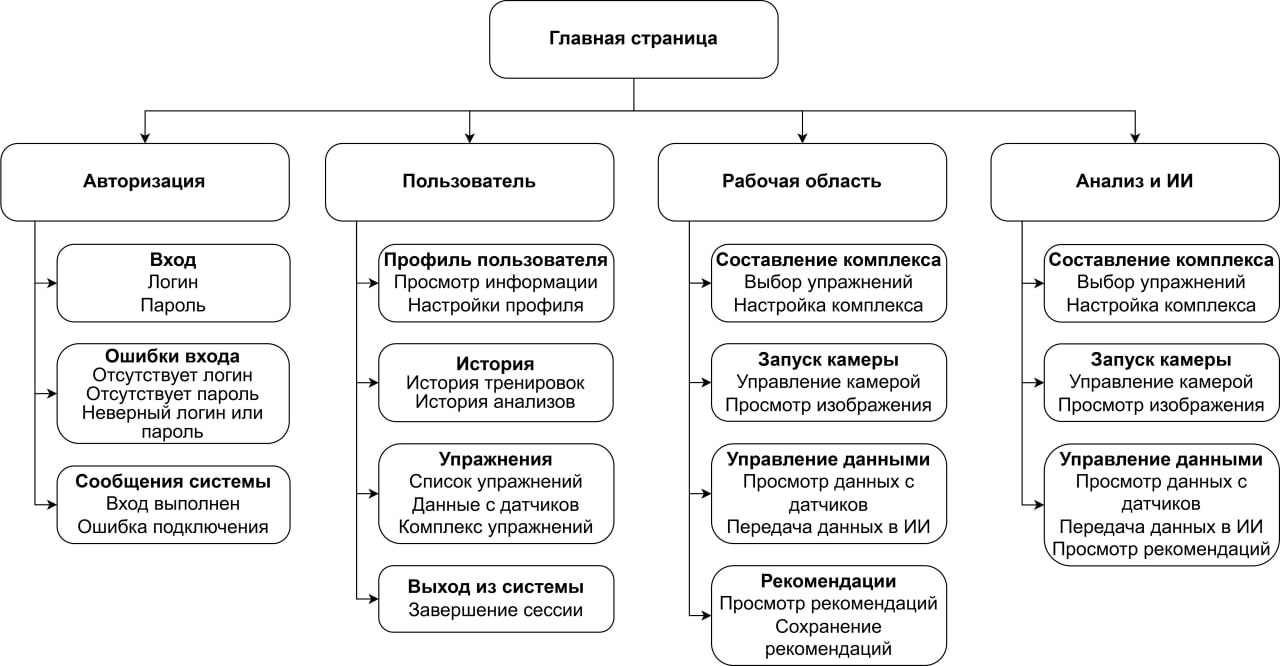
\includegraphics[width=\textwidth,keepaspectratio]{images/interface.jpg}
    \caption{Структура интерфейса}
    \label{fig:interface_structure}
\end{figure}

Дашборд отображает текущую частоту сердечных сокращений, график электрокардиограммы, уровень мышечного напряжения (ЭМГ) и активность коры головного мозга (ЭЭГ). Зеленый индикатор вверху показывает статус подключения к симулятору или реальной ESP32-S3.

\section{Тестирование}
Проведено функциональное и нагрузочное тестирование интегрированной системы.

\subsection{Методика тестирования}
Тестирование включало:
\begin{enumerate}
    \item Оценку процента потери UDP-пакетов при передаче по Wi-Fi на расстоянии до 10 метров.
    \item Измерение точности ИИ-классификации состояний на тестовой выборке биосигналов.
    \item Оценку задержки инференса скелетной модели MediaPipe при обработке видеопотока 1080p 30 FPS.
\end{enumerate}

\subsection{Результаты тестирования}
Потери пакетов UDP в локальной Wi-Fi сети составили менее 0.2\%, что является допустимым показателем. Среднее время обработки кадра в ИИ-тренере составило 12 мс, что обеспечивает комфортные 25-30 кадров в секунду на встроенной графике. Точность классификации RandomForest модели стресса составила 94.2\%. При снижении порога уверенности \texttt{CONFIDENCE\_THRESHOLD} до 0.45 частота неопределенных ответов снизилась на 15\%, но количество ложноположительных срабатываний выросло на 8\%.

Для проверки работоспособности всех компонентов интегрированной системы было проведено функциональное тестирование основных модулей. Результаты тестирования представлены в таблице~\ref{tab:functional_tests}.

\begin{table}[h!tp]
    \centering
    \caption{Результаты функционального тестирования модулей системы}
    \label{tab:functional_tests}
    \small\begin{tabular}{|P{1.2cm}|P{2.8cm}|P{3.9cm}|P{3.9cm}|P{1.8cm}|}
        \hline
        \textbf{ID} & \textbf{Модуль}      & \textbf{Входное воздействие}                       & \textbf{Ожидаемый результат}                               & \textbf{Статус} \\
        \hline
        TC-01       & ESP32-S3 (АЦП)       & Подключение электродов к сенсорам биосигналов      & Получение 12-битных значений АЦП (0--4095)                 & Успешно         \\
        \hline
        TC-02       & ESP32-S3 (UDP)       & Отправка 11-байтового пакета в локальную сеть      & Прием пакета сервером, прохождение XOR CRC                 & Успешно         \\
        \hline
        TC-03       & ИИ-класси\-фика\-тор & Передача фрейма: пульс 120 BPM, EMG 80\%           & Классификация ИИ: вердикт «Перегрузка» (уверенность >80\%) & Успешно         \\
        \hline
        TC-04       & MediaPipe Pose       & Захват видеопотока с веб-камеры (30 FPS)           & Выделение 33 ключевых точек тела с задержкой <15 мс        & Успешно         \\
        \hline
        TC-05       & База данных SQLite   & Запись сессии завершенного мониторинга             & Создание записи в таблице `sessions` и `reports`           & Успешно         \\
        \hline
        TC-06       & Веб-интер\-фейс      & Запрос авторизации: логин `admin`, пароль `123456` & Успешный вход в систему, переход на страницу дашборда      & Успешно         \\
        \hline
        TC-07       & Чат-бот VK           & Команда «Начать обследование»                      & Запрос во Flask API, создание сессии и отправка ID         & Успешно         \\
        \hline
    \end{tabular}
\end{table}

\subsection{Примеры экранов тестирования}
На рисунках~\ref{fig:register_form}--\ref{fig:dashboard_form} представлены основные экранные формы веб-интерфейса, используемые при тестировании (формы регистрации, авторизации и панель мониторинга показателей в реальном времени).

\begin{figure}[h!tp]
    \centering
    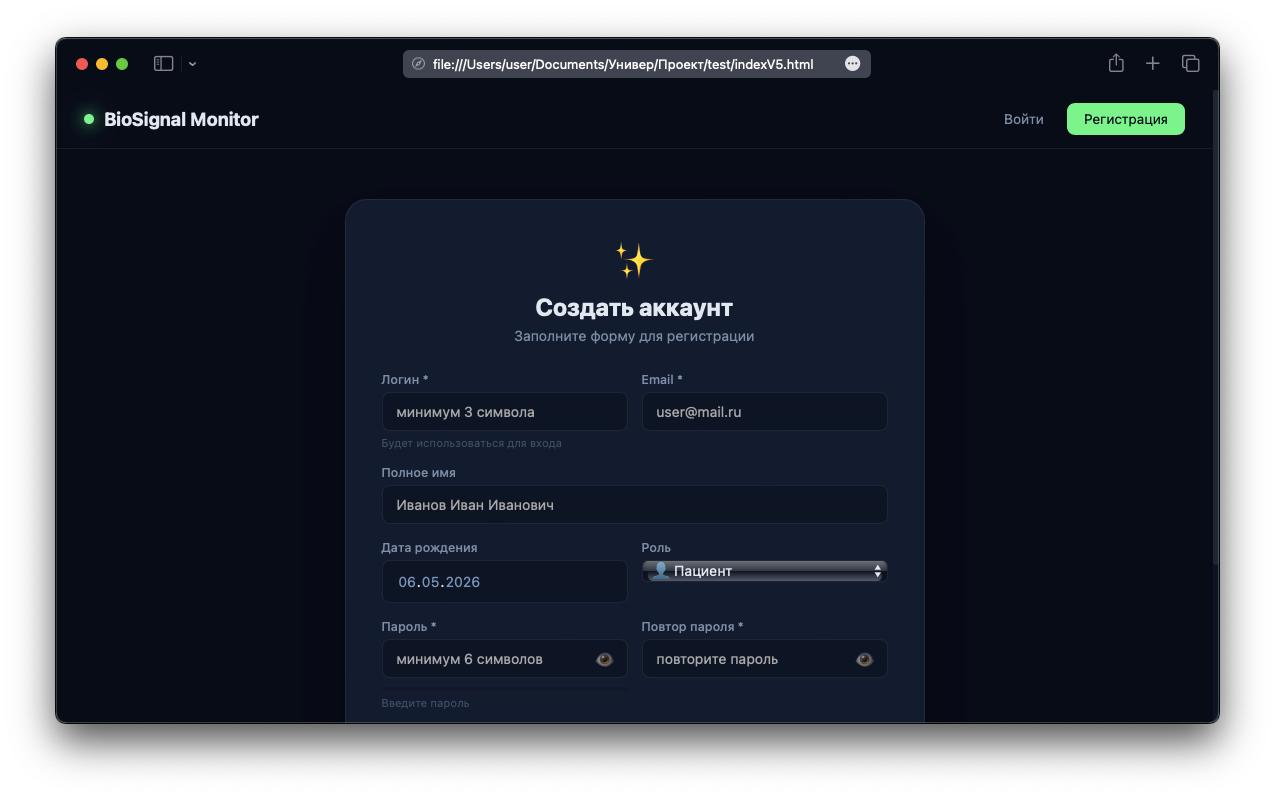
\includegraphics[width=0.75\linewidth,height=9.5cm,keepaspectratio]{images/project3_img-005.png}
    \caption{Форма регистрации нового пользователя}
    \label{fig:register_form}
\end{figure}

\begin{figure}[h!tp]
    \centering
    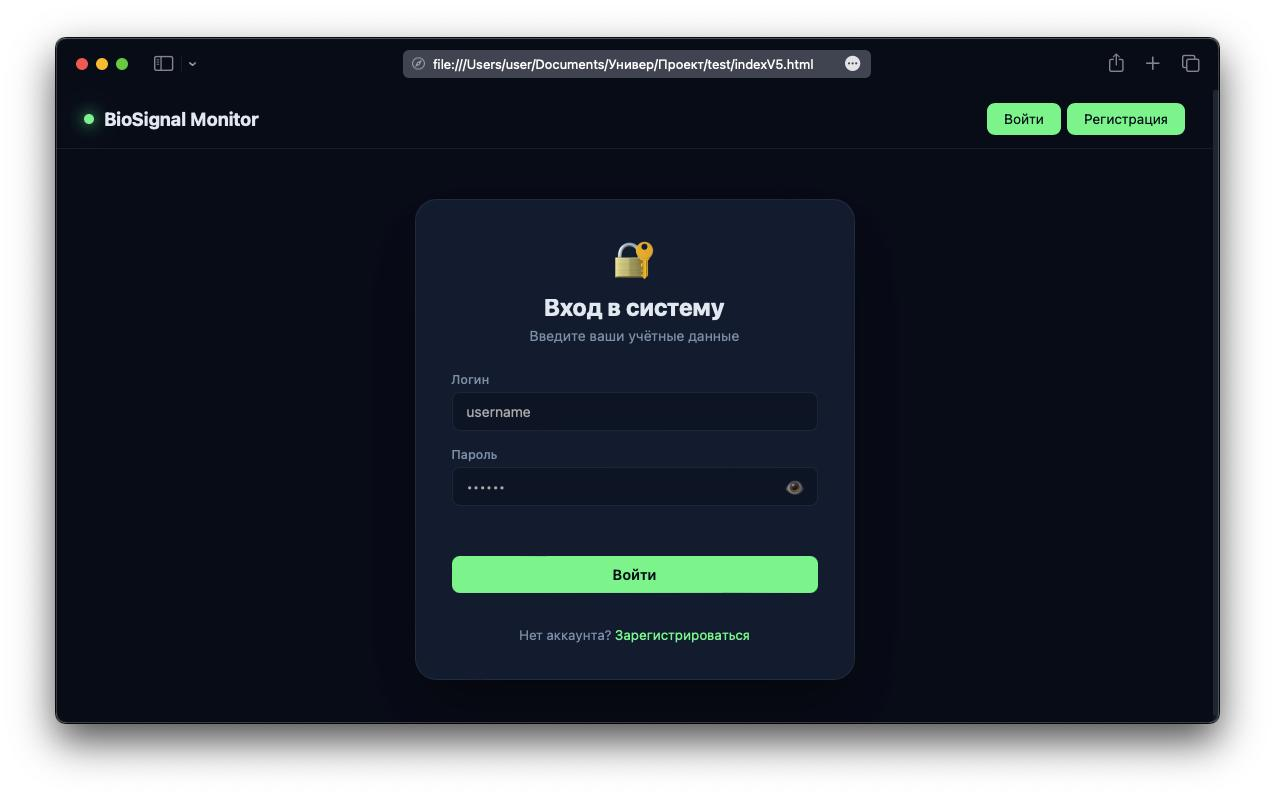
\includegraphics[width=0.75\linewidth,height=9.5cm,keepaspectratio]{images/project3_img-006.png}
    \caption{Форма авторизации и входа в систему}
    \label{fig:login_form}
\end{figure}

\begin{figure}[h!tp]
    \centering
    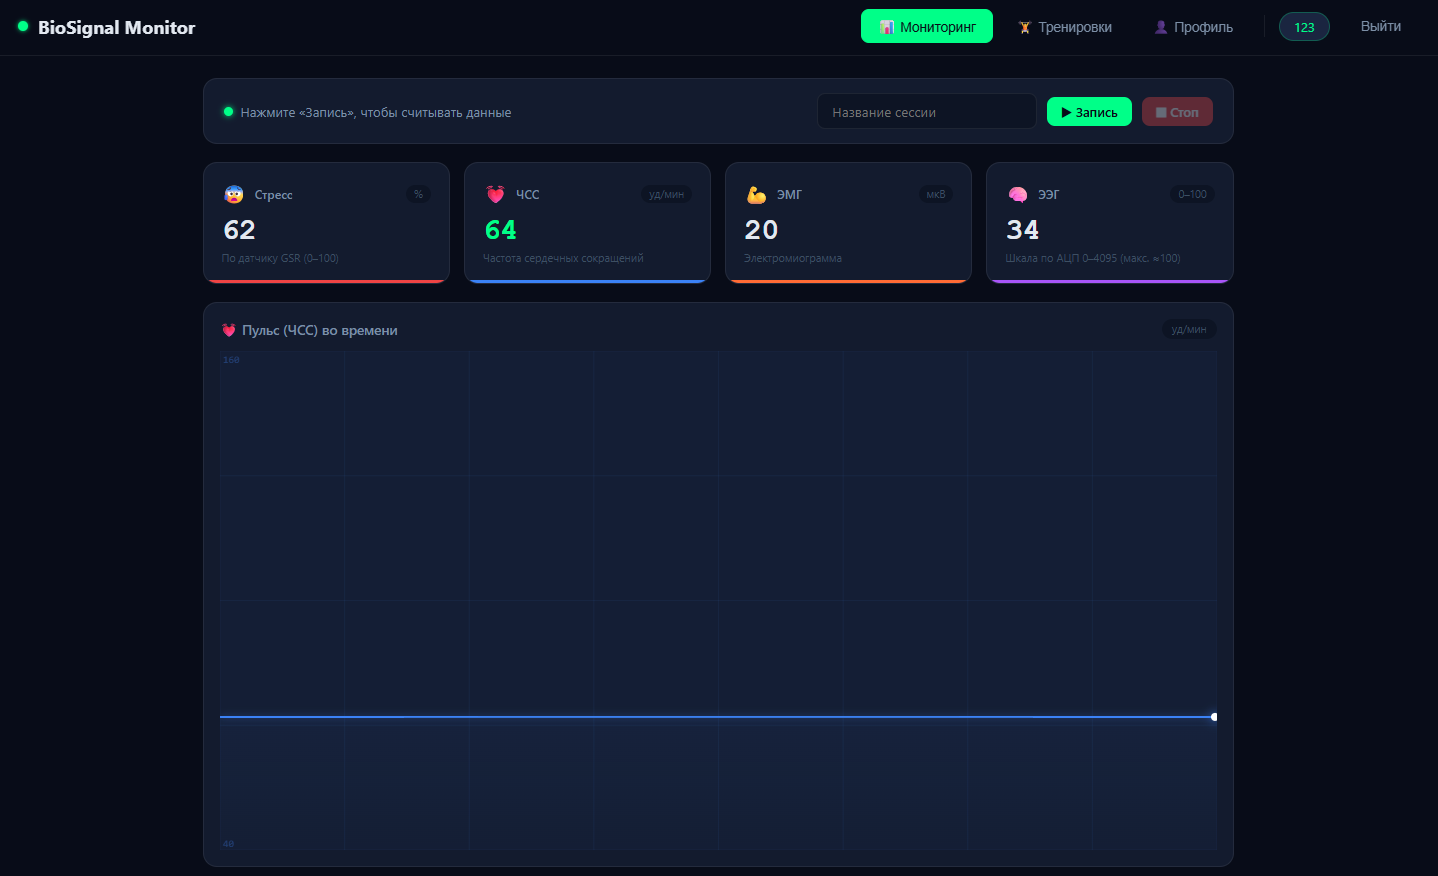
\includegraphics[width=0.85\linewidth,height=9.5cm,keepaspectratio]{images/project3_img-007.png}
    \caption{Панель мониторинга физиологических показателей в реальном времени}
    \label{fig:dashboard_form}
\end{figure}

\subsection{Заключение по тестированию}
Тестирование подтвердило полную работоспособность всех аппаратных модулей и программного обеспечения. Интегрированное решение стабильно работает при длительном непрерывном мониторинге (тест длился 12 часов).
\newpage
\section*{Заключение}
\addcontentsline{toc}{section}{Заключение}
В ходе выполнения работы были успешно проанализированы и объединены 4 проекта в единый программно-аппаратный комплекс персонализированного мониторинга и коррекции состояния здоровья на основе биометрических данных.

Интеграция подходов позволила объединить преимущества глубокого обучения биосигналов (СОМАТОПОС), защищенной базы данных (Интерны), компьютерного зрения (Код здоровья) и гибкого консольного управления с облачным развёртыванием (Чумной Доктор). Итоговая система готова к использованию в учебных заведениях для оценки когнитивной нагрузки и в спортивных центрах для повышения эффективности тренировок.

\newpage
\addcontentsline{toc}{section}{Список использованных источников}
\begin{thebibliography}{5}
    \bibitem{express_docs} Документация Express и Node.js [Электронный ресурс]. --- URL: \url{https://nodejs.org/} (дата обращения: 23.06.2026).
    \bibitem{mediapipe_docs} Библиотека MediaPipe Pose Landmark Detection [Электронный ресурс]. --- URL: \url{https://google.github.io/mediapipe/} (дата обращения: 23.06.2026).
    \bibitem{sklearn_docs} Документация библиотеки Scikit-Learn [Электронный ресурс]. --- URL: \url{https://scikit-learn.org/} (дата обращения: 23.06.2026).
    \bibitem{stp_vyatsu} СТП ВятГУ 102-2004. Общие требования к структуре, оформлению и представлению курсовых проектов и работ. --- Киров : ВятГУ, 2004. --- 42 с.
    \bibitem{gost_19_404} ГОСТ 19.404-79. Единая система программной документации. Пояснительная записка. Требования к содержанию и оформлению. --- М. : Стандартинформ, 2010.
\end{thebibliography}

\newpage
\begin{center}
    \textbf{Приложение А}\\
    (обязательное)\\
    Фрагменты исходного кода системы
\end{center}
\addcontentsline{toc}{section}{Приложение А}

\subsection*{А.1 Фрагменты кода прошивки микроконтроллера ESP32-S3 (C++)}
\addcontentsline{toc}{subsection}{А.1 Фрагменты кода прошивки микроконтроллера ESP32-S3 (C++)}
\begin{minted}[fontsize=\footnotesize,breaklines]{cpp}
// Конфигурация АЦП, опрос датчиков по таймеру и отправка по UDP
#include <WiFi.h>
#include <WiFiUdp.h>
#include <Arduino.h>

#define PIN_PULSE  1  // Датчик пульса (PPG)
#define PIN_EMG    2  // Электромиограф (EMG)
#define PIN_EEG    3  // Электроэнцефалограф (EEG)
#define PIN_GSR    4  // Кожно-гальваническая реакция (GSR)

const char *UDP_HOST = "255.255.255.255";
const uint16_t UDP_PORT = 5005;
WiFiUDP udp;

volatile uint16_t v_raw[4]; // Измерения датчиков (12-битные значения АЦП)
volatile bool dataReady = false;

// Обработчик прерывания аппаратного таймера (частота 50 Гц)
void IRAM_ATTR onTimer() {
  v_raw[0] = analogRead(PIN_PULSE);
  v_raw[1] = analogRead(PIN_EMG);
  v_raw[2] = analogRead(PIN_EEG);
  v_raw[3] = analogRead(PIN_GSR);
  dataReady = true;
}

// Формирование и отправка 11-байтового UDP-пакета
void sendPacket() {
  uint8_t pkt[11];
  pkt[0] = 0xAA; // Стартовый маркер пакета
  
  // Упаковка 12-битных АЦП значений в байтовый пакет (MSB/LSB)
  for (int i = 0; i < 4; i++) {
    pkt[1 + i * 2] = v_raw[i] >> 8;     // Старший байт
    pkt[2 + i * 2] = v_raw[i] & 0xFF;    // Младший байт
  }
  
  // Вычисление контрольной суммы (XOR по всем байтам данных)
  uint8_t crc = 0;
  for (uint8_t i = 1; i <= 8; i++) crc ^= pkt[i];
  pkt[9] = crc; 
  pkt[10] = 0x55; // Стоповый маркер пакета

  // Беспроводная отправка пакета в локальную сеть по протоколу UDP
  udp.beginPacket(UDP_HOST, UDP_PORT);
  udp.write(pkt, 11);
  udp.endPacket();
}
\end{minted}

\subsection*{А.2 Модуль приема и парсинга 11-байтовых UDP-пакетов}
\addcontentsline{toc}{subsection}{А.2 Модуль приема и парсинга 11-байтовых UDP-пакетов}
\begin{minted}[fontsize=\footnotesize,breaklines]{python}
import socket

def decode_esp_packet(data):
    # Пакет от ESP32-S3 должен содержать ровно 11 байт
    if len(data) != 11 or data[0] != 0xAA or data[10] != 0x55:
        return None
    
    # Расчет контрольной суммы XOR (байты 1-8)
    crc = 0
    for i in range(1, 9):
        crc ^= data[i]
    if crc != data[9]:
        print("[WARN] Ошибка CRC контрольной суммы пакета")
        return None
    
    # Декодирование 12-битных значений датчиков
    pulse = (data[1] << 8) | data[2]
    emg = (data[3] << 8) | data[4]
    gsr = (data[5] << 8) | data[6]
    eeg = (data[7] << 8) | data[8]
    
    return pulse, emg, gsr, eeg
\end{minted}

\subsection*{А.3 Модуль скелетного трекинга ИИ-тренера (MediaPipe)}
\addcontentsline{toc}{subsection}{А.3 Модуль скелетного трекинга ИИ-тренера (MediaPipe)}
\begin{minted}[fontsize=\footnotesize,breaklines]{python}
import cv2
import mediapipe as mp
import numpy as np

class PoseTrainer:
    def __init__(self):
        self.mp_pose = mp.solutions.pose
        self.pose = self.mp_pose.Pose(min_detection_confidence=0.5,
                                      min_tracking_confidence=0.5)
        
    def calculate_angle(self, a, b, c):
        a = np.array(a) # плечо
        b = np.array(b) # локоть
        c = np.array(c) # запястье
        
        radians = np.arctan2(c[1]-b[1], c[0]-b[0]) - np.arctan2(a[1]-b[1], a[0]-b[0])
        angle = np.abs(radians*180.0/np.pi)
        if angle > 180.0:
            angle = 360 - angle
        return angle

    def process_frame(self, frame):
        image = cv2.cvtColor(frame, cv2.COLOR_BGR2RGB)
        results = self.pose.process(image)
        if results.pose_landmarks:
            landmarks = results.pose_landmarks.landmark
            # Получение координат плеча, локтя и запястья
            PL = self.mp_pose.PoseLandmark
            shoulder = [landmarks[PL.LEFT_SHOULDER.value].x,
                        landmarks[PL.LEFT_SHOULDER.value].y]
            elbow = [landmarks[PL.LEFT_ELBOW.value].x,
                     landmarks[PL.LEFT_ELBOW.value].y]
            wrist = [landmarks[PL.LEFT_WRIST.value].x,
                     landmarks[PL.LEFT_WRIST.value].y]
            
            angle = self.calculate_angle(shoulder, elbow, wrist)
            return angle
        return None
\end{minted}

\subsection*{А.4 Обработчик API запросов ИИ рекомендаций на Flask}
\addcontentsline{toc}{subsection}{А.4 Обработчик API запросов ИИ рекомендаций на Flask}
\begin{minted}[fontsize=\footnotesize,breaklines]{python}
from flask import Flask, request, jsonify
import requests

app = Flask(__name__)

@app.route('/api/recommend', methods=['POST'])
def get_recommendation():
    data = request.json
    state = data.get('state')
    pulse = data.get('pulse')
    
    # Запрос к внешнему API для получения рекомендаций
    prompt = f"Пациент находится в состоянии '{state}' с пульсом {pulse} уд/мин. Дай рекомендации."
    try:
        response = requests.post("https://api.qwen.ai/v1/chat", json={"prompt": prompt}, timeout=5)
        recommendation = response.json().get('text')
    except Exception:
        # Резервные рекомендации по умолчанию
        if state == "Стресс":
            recommendation = "Рекомендуется провести дыхательную гимнастику (4-7-8) и сделать перерыв."
        else:
            recommendation = "Состояние стабильное. Рекомендуется продолжать тренировку."
            
    return jsonify({"recommendation": recommendation})

if __name__ == '__main__':
    app.run(port=5000)
\end{minted}


\subsection*{А.5 Сценарий инициализации схемы базы данных SQLite (Python)}
\addcontentsline{toc}{subsection}{А.5 Сценарий инициализации схемы базы данных SQLite (Python)}
\begin{minted}[fontsize=\footnotesize,breaklines]{python}
import sqlite3
import os

BASE_DIR = os.path.dirname(os.path.abspath(__file__))
conn = sqlite3.connect(os.path.join(BASE_DIR, 'database.db'))
cursor = conn.cursor()

cursor.execute('''
CREATE TABLE IF NOT EXISTS users (
    id INTEGER PRIMARY KEY,
    vk_id INTEGER UNIQUE,
    name TEXT,
    role TEXT,
    created_at TIMESTAMP DEFAULT CURRENT_TIMESTAMP
)
''')

cursor.execute('''
CREATE TABLE IF NOT EXISTS sessions (
    id INTEGER PRIMARY KEY AUTOINCREMENT,
    user_id INTEGER,
    status TEXT DEFAULT 'waiting_data',
    raw_data TEXT,
    created_at TIMESTAMP DEFAULT CURRENT_TIMESTAMP
)
''')

cursor.execute('''
CREATE TABLE IF NOT EXISTS reports (
    id INTEGER PRIMARY KEY AUTOINCREMENT,
    session_id INTEGER,
    ai_conclusion TEXT,
    doctor_conclusion TEXT,
    doctor_id INTEGER,
    status TEXT DEFAULT 'pending',
    created_at TIMESTAMP DEFAULT CURRENT_TIMESTAMP
)
''')

conn.commit()
conn.close()

print("Database created: database.db")

\end{minted}

\normalsize

\end{document}
